% ============================================================================
% Formal Safety and Liveness of DAG-Knight Consensus Under Partial Synchrony
% ============================================================================
\documentclass[11pt,a4paper]{article}

% ── Encoding & Fonts ────────────────────────────────────────────────────────
\usepackage[utf8]{inputenc}
\usepackage[T1]{fontenc}
\usepackage{lmodern}

% ── Mathematics ─────────────────────────────────────────────────────────────
\usepackage{amsmath,amssymb,amsthm,mathtools}

% ── Algorithms ──────────────────────────────────────────────────────────────
\usepackage{algorithm}
\usepackage{algpseudocode}

% ── Graphics & Diagrams ────────────────────────────────────────────────────
\usepackage{tikz}
\usepackage{pgfplots}
\pgfplotsset{compat=1.18}
\usetikzlibrary{shapes,arrows.meta,positioning,calc,decorations.pathmorphing,
                 backgrounds,fit,patterns}

% ── Tables & Formatting ────────────────────────────────────────────────────
\usepackage{booktabs}
\usepackage{array}
\usepackage{multirow}
\usepackage{tabularx}
\usepackage{enumitem}

% ── Colors ──────────────────────────────────────────────────────────────────
\usepackage{xcolor}
\definecolor{qblue}{RGB}{0,100,200}
\definecolor{qpurple}{RGB}{128,0,200}
\definecolor{qcyan}{RGB}{0,180,200}
\definecolor{qgreen}{RGB}{0,180,100}
\definecolor{qorange}{RGB}{255,140,0}
\definecolor{qred}{RGB}{220,50,50}
\definecolor{codebg}{RGB}{245,245,250}
\definecolor{darkblue}{RGB}{0,51,102}

% ── Code Listings ───────────────────────────────────────────────────────────
\usepackage{listings}
\lstset{
  backgroundcolor=\color{codebg},
  basicstyle=\small\ttfamily,
  keywordstyle=\color{qblue}\bfseries,
  commentstyle=\color{qgreen}\itshape,
  stringstyle=\color{qorange},
  numbers=left,
  numberstyle=\tiny\color{gray},
  frame=single,
  breaklines=true,
  captionpos=b
}

% ── Page Layout ─────────────────────────────────────────────────────────────
\usepackage[margin=1in]{geometry}
\usepackage{fancyhdr}
\pagestyle{fancy}
\fancyhead[L]{\textsc{DAG-Knight Formal Safety \& Liveness}}
\fancyhead[R]{\textsc{Q-NarwhalKnight}}
\fancyfoot[C]{\thepage}

% ── References ──────────────────────────────────────────────────────────────
\usepackage[colorlinks=true,linkcolor=darkblue,citecolor=qpurple,urlcolor=qblue]{hyperref}

% ── Theorem Environments ────────────────────────────────────────────────────
\newtheorem{theorem}{Theorem}[section]
\newtheorem{lemma}[theorem]{Lemma}
\newtheorem{corollary}[theorem]{Corollary}
\newtheorem{proposition}[theorem]{Proposition}
\newtheorem{claim}[theorem]{Claim}

\theoremstyle{definition}
\newtheorem{definition}[theorem]{Definition}
\newtheorem{assumption}[theorem]{Assumption}
\newtheorem{protocol}[theorem]{Protocol}

\theoremstyle{remark}
\newtheorem{remark}[theorem]{Remark}
\newtheorem{example}[theorem]{Example}

% ── Custom Commands ─────────────────────────────────────────────────────────
\newcommand{\DAG}{\textsf{DAG}}
\newcommand{\DK}{\textsf{DAG-Knight}}
\newcommand{\GST}{\mathrm{GST}}
\newcommand{\VDF}{\mathrm{VDF}}
\newcommand{\VRF}{\mathrm{VRF}}
\newcommand{\anticone}{\mathrm{anticone}}
\newcommand{\past}{\mathrm{past}}
\newcommand{\future}{\mathrm{future}}
\newcommand{\honest}{\mathcal{H}}
\newcommand{\byzantine}{\mathcal{B}}
\newcommand{\vertices}{\mathcal{V}}
\newcommand{\edges}{\mathcal{E}}
\newcommand{\round}{\mathsf{round}}
\newcommand{\anchor}{\mathsf{anchor}}
\newcommand{\commit}{\mathsf{commit}}
\newcommand{\order}{\prec}
\newcommand{\finalized}{\mathsf{finalized}}
\renewcommand{\kappa}{\varkappa}
\newcommand{\bigO}{\mathcal{O}}

% ============================================================================
\begin{document}

% ── Title ───────────────────────────────────────────────────────────────────
\begin{center}
{\LARGE\bfseries Formal Safety and Liveness of DAG-Knight\\
Consensus Under Partial Synchrony}

\vspace{0.8em}
{\large Q-NarwhalKnight Protocol Team}

\vspace{0.4em}
{\normalsize\texttt{research@quillon.xyz}}

\vspace{0.4em}
{\normalsize March 2026}

\vspace{0.4em}
{\small Version 2.0 (revised)}
\end{center}

% ── Abstract ────────────────────────────────────────────────────────────────
\begin{abstract}
We present a complete formal treatment of the \DK{} consensus protocol,
a DAG-based Byzantine fault-tolerant (BFT) ordering protocol that operates
under the partial synchrony model of Dwork, Lynch, and Stockmeyer.
\DK{} constructs a directed acyclic graph of \emph{vertices} proposed by
validators, elects \emph{anchor} vertices via a VDF-based lottery on even rounds,
and commits vertices through a $\delta$-round delayed commit rule.

We prove two main results.
\textbf{Theorem~\ref{thm:safety} (Safety):}
no two honest validators ever finalize conflicting total orderings of the
vertex set, even during asynchronous periods before the Global Stabilization
Time~$\GST$.
\textbf{Theorem~\ref{thm:liveness} (Liveness):}
after~$\GST$, every transaction submitted by an honest client is finalized
within $\bigO(\delta \cdot \Delta)$ time, where~$\delta$ is the commit-rule
depth and~$\Delta$ is the known message-delay bound.

We further derive a \emph{phase-transition} result for the connectivity
parameter~$\kappa = \lfloor 2\delta\Lambda / D \rfloor$: when $\kappa$
exceeds a critical threshold~$\kappa_c$, the DAG is sufficiently connected
to guarantee unique anchor election and deterministic ordering with
overwhelming probability.
A comparative analysis shows that \DK{} achieves $\bigO(\delta \cdot \Delta)$
finality under partial synchrony, compared to
PHANTOM's $\bigO(\kappa \Delta \log(1/\varepsilon))$ under synchrony
and GhostDAG's $\bigO(\kappa \Delta)$ under synchrony; we discuss the
trade-offs inherent in comparing across different network models.
Finally, we introduce a topological health-monitoring mechanism that uses
connected-component counting ($\beta_0$) for partition detection and a
tip-counting heuristic for fork detection, providing lightweight real-time
DAG diagnostics.
\end{abstract}

\tableofcontents
\newpage

% ============================================================================
% SECTION 1: INTRODUCTION
% ============================================================================
\section{Introduction}\label{sec:intro}

Distributed consensus---the problem of getting a set of mutually distrustful
nodes to agree on a total ordering of transactions---lies at the foundation
of every blockchain system.
Classical BFT protocols such as PBFT~\cite{castro1999pbft} achieve safety
and liveness under $n \geq 3f+1$ with $f$ Byzantine faults, but their
$\bigO(n^2)$ message complexity limits practical deployments to tens of
validators.
DAG-based protocols~\cite{sompolinsky2021phantom,sompolinsky2018spectre}
amortize communication costs by embedding transactions in a DAG of
\emph{vertices} linked via causal references, achieving near-linear
message complexity while retaining BFT guarantees.

The \DK{} protocol~\cite{sompolinsky2022dagknight} advances the DAG
paradigm by introducing a parameterized ordering rule whose security
depends on a single connectivity parameter~$\kappa$ rather than a fixed
block-creation rate.
However, existing analyses~\cite{sompolinsky2022dagknight} leave several
gaps: (i)~no formal proof of safety during pre-$\GST$ asynchronous periods,
(ii)~no explicit liveness bound expressed in terms of the partial synchrony
parameters, and (iii)~no treatment of the $\kappa$ phase transition in a
rigorous probabilistic framework.

\subsection{Contributions}

This paper addresses these gaps with the following contributions:

\begin{enumerate}[leftmargin=*]
\item \textbf{Safety (Theorem~\ref{thm:safety}):}
  We prove that no two honest validators finalize conflicting orderings,
  building on three structural lemmas: unique anchor election
  (Lemma~\ref{lem:unique-anchor}), unique commit determination
  (Lemma~\ref{lem:unique-commit}), and deterministic ordering
  (Lemma~\ref{lem:deterministic-ordering}).

\item \textbf{Asynchronous safety (Theorem~\ref{thm:async-safety}):}
  Safety holds even before~$\GST$, when message delays are unbounded,
  because the commit rule is purely local and does not depend on timing
  assumptions.

\item \textbf{Tail-fork resistance (Theorem~\ref{thm:tail-fork}):}
  We formalize the tail-fork attack and prove that the $\delta$-round
  commit rule with ancestor finality checks prevents conflicting proposals
  for unfinalized rounds.

\item \textbf{Liveness (Theorem~\ref{thm:liveness}):}
  After~$\GST$, every honest transaction is finalized within
  $T \leq 3\Delta + 2\epsilon$ time for $\delta = 1$, where $\epsilon$
  is local processing overhead.

\item \textbf{$\kappa$-parameter phase transition (Theorem~\ref{thm:kappa}):}
  We derive a critical threshold $\kappa_c$ above which the DAG's
  connectivity is sufficient for unique ordering with probability
  $\geq 1 - e^{-\Omega(\kappa)}$.

\item \textbf{Comparative analysis (Section~\ref{sec:comparison}):}
  We compare \DK{}'s finality guarantees against PHANTOM and GhostDAG,
  noting that \DK{} achieves deterministic safety under partial synchrony
  while the latter protocols provide probabilistic safety under synchrony.
  We discuss when and why direct comparison of finality bounds across
  models is and is not meaningful.

\item \textbf{Topological health monitoring (Section~\ref{sec:homology}):}
  We introduce connected-component counting ($\beta_0$) for partition
  detection and a tip-counting heuristic for fork estimation, providing
  lightweight DAG diagnostics.
  We prove correctness of the $\beta_0$ predicate and characterize the
  tip-counting approximation's limitations.
\end{enumerate}

\subsection{Paper Organization}

Section~\ref{sec:model} defines the system model.
Section~\ref{sec:protocol} specifies the \DK{} protocol.
Sections~\ref{sec:safety} and~\ref{sec:liveness} present safety and
liveness proofs.
Section~\ref{sec:kappa} analyzes the $\kappa$-parameter.
Section~\ref{sec:comparison} compares with related DAG protocols.
Section~\ref{sec:homology} develops the homological fork detection theory.
Section~\ref{sec:discussion} discusses implementation considerations.
Section~\ref{sec:related} surveys related work, and
Section~\ref{sec:conclusion} concludes.

% ============================================================================
% SECTION 2: SYSTEM MODEL
% ============================================================================
\section{System Model}\label{sec:model}

\subsection{Network and Timing}

We adopt the partial synchrony model of Dwork, Lynch, and
Stockmeyer~\cite{dwork1988consensus}.

\begin{assumption}[Partial Synchrony]\label{asm:partial-sync}
There exists an unknown Global Stabilization Time $\GST \geq 0$ and a
known bound $\Delta > 0$ such that any message sent by an honest validator
at time $t \geq \GST$ arrives at every honest validator by time
$t + \Delta$.
Before $\GST$, message delays are arbitrary but finite.
\end{assumption}

\begin{assumption}[Byzantine Threshold]\label{asm:byz}
The system consists of $n = 3f + 1$ validators, of which at most $f$ are
Byzantine.
Byzantine validators may deviate arbitrarily from the protocol; honest
validators follow the protocol faithfully.
\end{assumption}

\begin{definition}[Honest Majority Quorum]\label{def:quorum}
A \emph{quorum} $Q \subseteq \{1, \ldots, n\}$ satisfies $|Q| \geq 2f+1$.
The \emph{honest core} of a quorum is $Q \cap \honest$, where $\honest$
denotes the set of honest validators.
\end{definition}

\begin{lemma}[Quorum Intersection]\label{lem:quorum-intersection}
For any two quorums $Q_1, Q_2$ with $|Q_1|, |Q_2| \geq 2f+1$ and
$n = 3f+1$:
\[
  |Q_1 \cap Q_2 \cap \honest| \geq 1.
\]
\end{lemma}

\begin{proof}
We have $|Q_1 \cap Q_2| \geq |Q_1| + |Q_2| - n \geq (2f+1) + (2f+1) -
(3f+1) = f+1$.
Since at most $f$ validators are Byzantine,
$|Q_1 \cap Q_2 \cap \honest| \geq (f+1) - f = 1$.
\end{proof}

\subsection{DAG Structure}

\begin{definition}[Vertex]\label{def:vertex}
A \emph{vertex} $v = (\mathsf{id}, \mathsf{author}, \round(v),
\mathsf{parents}(v), \mathsf{payload}(v), \sigma_v)$ consists of:
\begin{itemize}[nosep]
  \item $\mathsf{id} \in \{0,1\}^{256}$: a cryptographic hash of the
    vertex contents;
  \item $\mathsf{author} \in \{1, \ldots, n\}$: the proposing validator;
  \item $\round(v) \in \mathbb{N}$: the protocol round;
  \item $\mathsf{parents}(v) \subseteq \vertices$: references to
    vertices from round $\round(v) - 1$ (at least $2f+1$ parents
    required from honest validators);
  \item $\mathsf{payload}(v)$: a batch of client transactions;
  \item $\sigma_v$: a digital signature by $\mathsf{author}$.
\end{itemize}
\end{definition}

\begin{definition}[DAG]\label{def:dag}
The \emph{protocol DAG} $G = (\vertices, \edges)$ is defined by
$\vertices = \bigcup_{r \geq 0} V_r$ where $V_r$ is the set of vertices
in round~$r$, and $(u, v) \in \edges$ iff $u \in \mathsf{parents}(v)$.
\end{definition}

\begin{definition}[Causal History]\label{def:causal-past}
The \emph{causal past} of vertex~$v$ is
$\past(v) = \{u \in \vertices \mid \text{there is a directed path from } u \text{ to } v\}$.
The \emph{anticone} of $v$ is
$\anticone(v) = \vertices \setminus (\past(v) \cup \future(v) \cup \{v\})$.
\end{definition}

\begin{definition}[Certificate]\label{def:certificate}
A \emph{round-$r$ certificate} for validator~$i$ is a set
$C_r^{(i)} \subseteq V_r^{(i)}$ of vertices from at least $2f+1$
distinct validators in round~$r$ that validator~$i$ has locally delivered.
A certificate is a \emph{local observation}: each validator forms its own
certificate once it has received sufficiently many round-$r$ vertices.
Two honest validators' certificates $C_r^{(i)}$ and $C_r^{(j)}$ are not
necessarily identical, but by Lemma~\ref{lem:quorum-intersection} they
share at least one honest validator's vertex.
\end{definition}

\begin{remark}[Certificate agreement]\label{rem:certificate-agreement}
Certificates are \emph{not} signed aggregate objects (unlike threshold
certificates in HotStuff~\cite{yin2019hotstuff}).
Agreement on the committed vertex set is achieved not through certificate
identity but through the anchor election's view-synchronization mechanism
(Section~\ref{sec:anchor-election}).
\end{remark}

\begin{figure}[t]
\centering
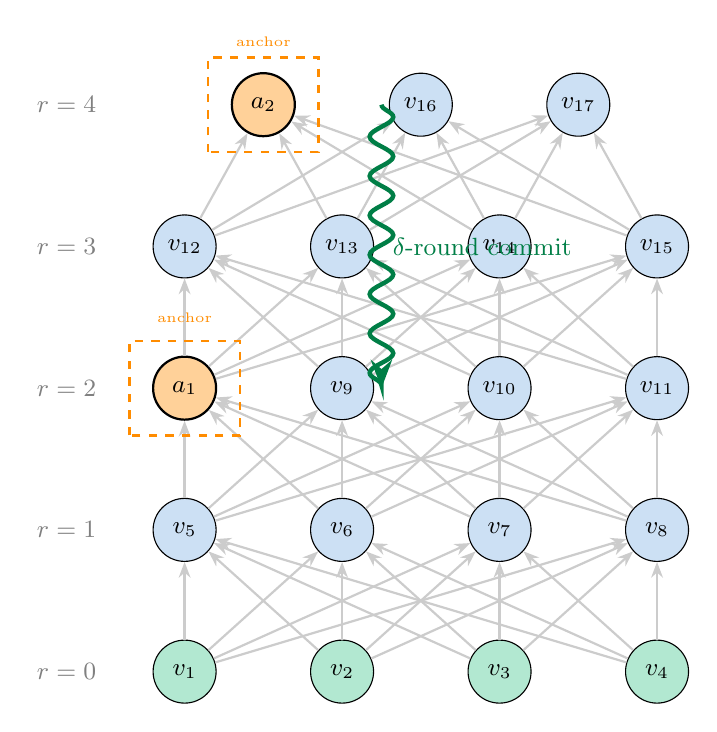
\begin{tikzpicture}[
    vertex/.style={circle, draw, fill=qblue!20, minimum size=8mm, font=\small},
    anchor_v/.style={circle, draw, fill=qorange!40, minimum size=8mm, font=\small, thick},
    committed/.style={circle, draw, fill=qgreen!30, minimum size=8mm, font=\small},
    edge/.style={-{Stealth[length=2mm]}, thick},
    round_label/.style={font=\small\bfseries, text=gray}
]

% Round labels
\node[round_label] at (-1.5, 0) {$r=0$};
\node[round_label] at (-1.5, 1.8) {$r=1$};
\node[round_label] at (-1.5, 3.6) {$r=2$};
\node[round_label] at (-1.5, 5.4) {$r=3$};
\node[round_label] at (-1.5, 7.2) {$r=4$};

% Round 0 (committed)
\node[committed] (v00) at (0, 0) {$v_1$};
\node[committed] (v01) at (2, 0) {$v_2$};
\node[committed] (v02) at (4, 0) {$v_3$};
\node[committed] (v03) at (6, 0) {$v_4$};

% Round 1
\node[vertex] (v10) at (0, 1.8) {$v_5$};
\node[vertex] (v11) at (2, 1.8) {$v_6$};
\node[vertex] (v12) at (4, 1.8) {$v_7$};
\node[vertex] (v13) at (6, 1.8) {$v_8$};

% Round 2 (anchor round)
\node[anchor_v] (v20) at (0, 3.6) {$a_1$};
\node[vertex] (v21) at (2, 3.6) {$v_9$};
\node[vertex] (v22) at (4, 3.6) {$v_{10}$};
\node[vertex] (v23) at (6, 3.6) {$v_{11}$};

% Round 3
\node[vertex] (v30) at (0, 5.4) {$v_{12}$};
\node[vertex] (v31) at (2, 5.4) {$v_{13}$};
\node[vertex] (v32) at (4, 5.4) {$v_{14}$};
\node[vertex] (v33) at (6, 5.4) {$v_{15}$};

% Round 4 (anchor round)
\node[anchor_v] (v40) at (1, 7.2) {$a_2$};
\node[vertex] (v41) at (3, 7.2) {$v_{16}$};
\node[vertex] (v42) at (5, 7.2) {$v_{17}$};

% Edges (subset shown for clarity)
\foreach \child in {v10,v11,v12,v13} {
  \foreach \parent in {v00,v01,v02,v03} {
    \draw[edge, gray!40] (\parent) -- (\child);
  }
}
\foreach \child in {v20,v21,v22,v23} {
  \foreach \parent in {v10,v11,v12,v13} {
    \draw[edge, gray!40] (\parent) -- (\child);
  }
}
\foreach \child in {v30,v31,v32,v33} {
  \foreach \parent in {v20,v21,v22,v23} {
    \draw[edge, gray!40] (\parent) -- (\child);
  }
}
\foreach \child in {v40,v41,v42} {
  \draw[edge, gray!40] (v30) -- (\child);
  \draw[edge, gray!40] (v31) -- (\child);
  \draw[edge, gray!40] (v32) -- (\child);
  \draw[edge, gray!40] (v33) -- (\child);
}

% Anchor highlights
\draw[qorange, thick, dashed] (-0.7, 3.0) rectangle (0.7, 4.2);
\node[font=\tiny, text=qorange] at (0, 4.5) {anchor};

\draw[qorange, thick, dashed] (0.3, 6.6) rectangle (1.7, 7.8);
\node[font=\tiny, text=qorange] at (1, 8.0) {anchor};

% Commit arrow
\draw[-{Stealth}, ultra thick, qgreen!70!black, decorate,
      decoration={snake, amplitude=1.5mm, segment length=5mm}]
      (2.5, 7.2) -- node[right, font=\small] {$\delta$-round commit} (2.5, 3.6);

\end{tikzpicture}
\caption{DAG structure with 4 validators across 5 rounds.
Orange vertices are elected anchors (even rounds only).
Green vertices are committed.
The $\delta$-round commit rule at round~4 finalizes vertices up to round~$4 - \delta$.}
\label{fig:dag-structure}
\end{figure}

% ============================================================================
% SECTION 3: PROTOCOL SPECIFICATION
% ============================================================================
\section{Protocol Specification}\label{sec:protocol}

The \DK{} protocol proceeds in discrete rounds.
Each validator proposes at most one vertex per round, referencing $\geq 2f+1$
vertices from the previous round as parents.
The protocol comprises four components: (i)~vertex proposal and
dissemination, (ii)~anchor election on even rounds, (iii)~the $\delta$-round
commit rule, and (iv)~deterministic total ordering.

\subsection{Vertex Proposal}\label{sec:vertex-proposal}

\begin{protocol}[Vertex Proposal]\label{prot:proposal}
At the beginning of round~$r$, each honest validator~$i$:
\begin{enumerate}[nosep]
  \item Waits until it has received vertices from $\geq 2f+1$ distinct
    validators for round $r-1$.
  \item Constructs vertex $v$ with $\round(v) = r$,
    $\mathsf{parents}(v) \supseteq C_{r-1}$ (a round-$(r\!-\!1)$ certificate),
    and $\mathsf{payload}(v)$ containing pending client transactions.
  \item Signs $v$ and broadcasts it to all validators via reliable broadcast.
\end{enumerate}
\end{protocol}

\begin{remark}\label{rem:reliable-broadcast}
The reliable broadcast primitive (Bracha's protocol~\cite{bracha1987asynchronous})
ensures that if an honest validator delivers vertex~$v$, then all honest
validators \emph{eventually} deliver~$v$.
\textbf{Caveat:} ``eventually'' provides no timing guarantee before~$\GST$.
Two honest validators may form round-$r$ certificates at arbitrarily
different times during asynchronous periods.
Safety holds regardless of this timing gap (Theorem~\ref{thm:async-safety}),
but liveness requires bounded delivery after~$\GST$.
\end{remark}

\subsection{Anchor Election}\label{sec:anchor-election}

Anchors serve as ``leaders'' that define commit points in the DAG.
\DK{} elects anchors only on even rounds, using a VDF-based lottery
that is deterministic, verifiable, and non-manipulable.

\begin{definition}[VDF-Based Anchor Election]\label{def:anchor-election}
For even round~$r$, the anchor election proceeds as:
\begin{enumerate}[nosep]
  \item Compute a \emph{quantum beacon}:
    $\beta_r = H(\texttt{"beacon"} \| r \| \mathsf{entropy}_r)$,
    where $H$ is SHA3-256 and $\mathsf{entropy}_r$ is a deterministic
    seed derived from the round number.
  \item For each candidate vertex $v \in V_r$, compute a VDF challenge:
    $c_v = H(v.\mathsf{id} \| \beta_r \| r)$.
  \item Evaluate the VDF: $(\pi_v, y_v) = \VDF.\mathsf{Eval}(c_v, T)$,
    where $T$ is the difficulty parameter.
  \item Select the anchor: $\anchor(r) = \arg\min_{v \in V_r} y_v$.
\end{enumerate}
\end{definition}

\begin{definition}[Certified Candidate Set]\label{def:certified-candidates}
A round-$r$ vertex $v$ is \emph{certified} at validator~$i$ if $v$ appears
as a parent of at least $f+1$ round-$(r\!+\!1)$ vertices in $i$'s local DAG.
The \emph{certified candidate set} is:
\[
  V_r^{\star(i)} = \{v \in V_r^{(i)} \mid v \text{ is a parent of } \geq f+1 \text{ vertices in } V_{r+1}^{(i)}\}.
\]
The anchor election (Definition~\ref{def:anchor-election}) is evaluated
over $V_r^{\star(i)}$ rather than the full view $V_r^{(i)}$.
\end{definition}

\begin{lemma}[View Synchronization]\label{lem:view-sync}
For any even round~$r$ and any two honest validators $i, j$ that both
form round-$(r\!+\!1)$ certificates, the certified candidate sets are identical:
$V_r^{\star(i)} = V_r^{\star(j)}$.
\end{lemma}

\begin{proof}
Let $v \in V_r^{\star(i)}$, so $v$ is referenced by $\geq f+1$
round-$(r\!+\!1)$ vertices in $i$'s DAG.
Since at most $f$ validators are Byzantine, at least one of these
$f+1$ referencing vertices was created by an honest validator~$h$.
Honest validator~$h$ only references $v$ if~$h$ delivered~$v$.
By reliable broadcast (Remark~\ref{rem:reliable-broadcast}), all honest
validators---including~$j$---eventually deliver~$v$, so
$v \in V_r^{(j)}$.

Moreover, since~$j$ forms a round-$(r\!+\!1)$ certificate (receiving
$\geq 2f+1$ round-$(r\!+\!1)$ vertices), at least $f+1$ of these are
honest.
Each honest round-$(r\!+\!1)$ validator delivered~$v$ (by the argument above)
and references~$v$ as a parent, so $v$ is referenced by $\geq f+1$
round-$(r\!+\!1)$ vertices in $j$'s DAG.
Hence $v \in V_r^{\star(j)}$.
By symmetry, $V_r^{\star(j)} \subseteq V_r^{\star(i)}$.
\end{proof}

\begin{lemma}[Anchor Uniqueness]\label{lem:anchor-unique-def}
For any even round~$r$, if $|V_r^{\star}| \geq 2f+1$, then the anchor
$\anchor(r) = \arg\min_{v \in V_r^{\star}} y_v$ is uniquely determined.
\end{lemma}

\begin{proof}
The VDF output $y_v$ is a 256-bit value.
The probability that two distinct vertices $v \neq w$ satisfy $y_v = y_w$
is $2^{-256}$, which is negligible.
Since $\arg\min$ over distinct values is unique, the anchor is uniquely
determined.
\end{proof}

\begin{figure}[t]
\centering
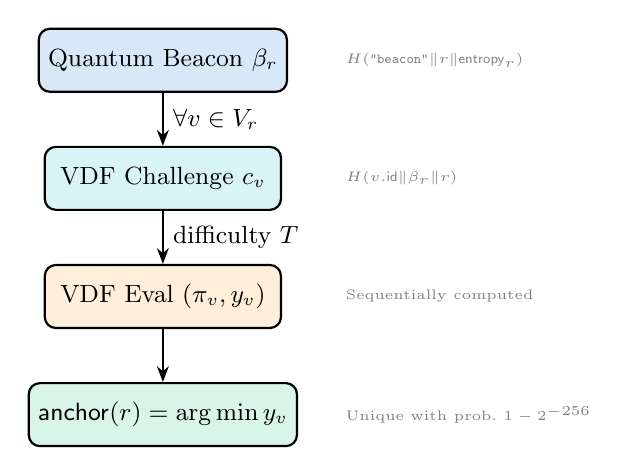
\begin{tikzpicture}[
    box/.style={draw, rounded corners, minimum width=3cm, minimum height=0.8cm,
                font=\small, thick},
    arr/.style={-{Stealth[length=2mm]}, thick}
]

\node[box, fill=qblue!15] (beacon) at (0, 0) {Quantum Beacon $\beta_r$};
\node[box, fill=qcyan!15] (challenge) at (0, -1.5) {VDF Challenge $c_v$};
\node[box, fill=qorange!15] (eval) at (0, -3.0) {VDF Eval $(\pi_v, y_v)$};
\node[box, fill=qgreen!15] (select) at (0, -4.5) {$\anchor(r) = \arg\min y_v$};

\draw[arr] (beacon) -- (challenge) node[midway, right, font=\small]
    {$\forall v \in V_r$};
\draw[arr] (challenge) -- (eval) node[midway, right, font=\small]
    {difficulty $T$};
\draw[arr] (eval) -- (select);

\node[font=\tiny, text=gray, right] at (2.2, 0) {$H(\texttt{"beacon"} \| r \| \mathsf{entropy}_r)$};
\node[font=\tiny, text=gray, right] at (2.2, -1.5) {$H(v.\mathsf{id} \| \beta_r \| r)$};
\node[font=\tiny, text=gray, right] at (2.2, -3.0) {Sequentially computed};
\node[font=\tiny, text=gray, right] at (2.2, -4.5) {Unique with prob.\ $1 - 2^{-256}$};

\end{tikzpicture}
\caption{VDF-based anchor election pipeline for even round~$r$.}
\label{fig:anchor-election}
\end{figure}

\subsection{The $\delta$-Round Commit Rule}\label{sec:commit-rule}

The commit rule determines when vertices become finalized.
\DK{} uses a $\delta$-round delayed commit: vertices in round~$r$ are
committed when a valid anchor is elected at round~$r + \delta$.

\begin{definition}[$\delta$-Round Commit]\label{def:delta-commit}
Let $\delta \geq 1$ be the commit depth parameter.
When an anchor $\anchor(r)$ is elected at even round~$r$, all vertices
in round $r - \delta$ and below are \emph{committed}.
Formally, for all $v$ with $\round(v) \leq r - \delta$:
\[
  \finalized(v) \leftarrow \texttt{true}.
\]
\end{definition}

\begin{definition}[Finality State]\label{def:finality-state}
A vertex $v$ is in one of three states:
\begin{itemize}[nosep]
  \item \textbf{Pending}: $v$ has been proposed but not yet committed.
  \item \textbf{Committed}: $v$ has been committed by the $\delta$-round rule.
  \item \textbf{Finalized}: $v$ is committed and its total ordering position
    is determined.
\end{itemize}
\end{definition}

\begin{protocol}[Commit Evaluation]\label{prot:commit}
Upon receiving an anchor election result for even round~$r$:
\begin{enumerate}[nosep]
  \item If $r < \delta$, skip (insufficient history).
  \item Set $r_c = r - \delta$ (the commit round).
  \item For all vertices $v$ with $\round(v) \leq r_c$ that are not
    yet committed: set $\finalized(v) \leftarrow \texttt{true}$.
  \item Invoke the deterministic ordering procedure
    (Section~\ref{sec:ordering}) on the newly committed vertices.
\end{enumerate}
\end{protocol}

\subsection{Tail-Fork Protection}\label{sec:tail-fork-protocol}

A \emph{tail fork} occurs when a Byzantine validator proposes two
conflicting vertices for the same round, attempting to create ambiguity
in the uncommitted tail of the DAG.

\begin{definition}[Tail Fork]\label{def:tail-fork}
A tail fork at round~$r$ exists when there are two vertices
$v_1, v_2 \in V_r$ with $v_1.\mathsf{author} = v_2.\mathsf{author}$
and $v_1.\mathsf{id} \neq v_2.\mathsf{id}$ in the uncommitted region
$[\text{last committed round}, r]$.
\end{definition}

\begin{protocol}[Proposal Safety Validation]\label{prot:tail-fork}
Before proposing vertex~$v$ for round~$r$, validator~$i$ checks:
\begin{enumerate}[nosep]
  \item \textbf{Parent committed}: At least one parent of $v$ is in
    a committed round. (Warning if violated, but allowed.)
  \item \textbf{No conflict}: No other vertex by $i$ exists for round~$r$.
    (Reject if violated.)
  \item \textbf{Ancestor finality}: The parent vertex has a valid anchor
    in its causal past. (Reject if violated.)
\end{enumerate}
\end{protocol}

\subsection{Deterministic Total Ordering}\label{sec:ordering}

\begin{definition}[Topological Ordering with Hash Tie-Breaking]\label{def:ordering}
The total ordering $\order$ on committed vertices is computed as follows:
\begin{enumerate}[nosep]
  \item \textbf{Round ordering}: If $\round(u) < \round(v)$, then $u \order v$.
  \item \textbf{Causal ordering}: Within the same round, if $u \in \past(v)$,
    then $u \order v$.
  \item \textbf{Hash tie-breaking}: For vertices $u, v$ in the same round
    with no causal relationship, order by
    $u \order v \iff u.\mathsf{id} < v.\mathsf{id}$
    (lexicographic comparison of hashes).
\end{enumerate}
\end{definition}

\begin{lemma}[Ordering is a Total Order]\label{lem:total-order}
The relation $\order$ defined above is a strict total order on~$\vertices$.
\end{lemma}

\begin{proof}
\emph{Irreflexivity}: A vertex cannot precede itself since $\round(v) \not< \round(v)$
and $v.\mathsf{id} \not< v.\mathsf{id}$.
\emph{Transitivity}: Follows from transitivity of $<$ on $\mathbb{N}$
(rounds), causal paths (DAG reachability), and lexicographic order (hashes).
\emph{Totality}: For any $u \neq v$, either $\round(u) \neq \round(v)$
(resolved by round ordering) or $\round(u) = \round(v)$ and either
$u \in \past(v)$, $v \in \past(u)$ (resolved causally), or neither
(resolved by hash comparison, unique since $u.\mathsf{id} \neq v.\mathsf{id}$).
\end{proof}

\begin{figure}[t]
\centering
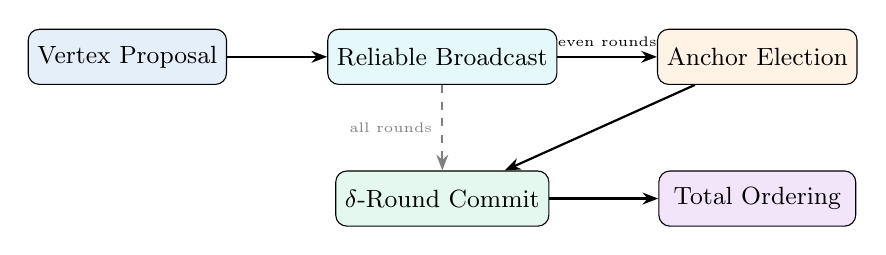
\begin{tikzpicture}[
    box/.style={draw, rounded corners, fill=white, minimum width=2.5cm,
                minimum height=0.7cm, font=\small},
    arr/.style={-{Stealth[length=2mm]}, thick}
]

% Ordering pipeline
\node[box, fill=qblue!10] (propose) at (0, 0) {Vertex Proposal};
\node[box, fill=qcyan!10] (broadcast) at (4, 0) {Reliable Broadcast};
\node[box, fill=qorange!10] (anchor) at (8, 0) {Anchor Election};
\node[box, fill=qgreen!10] (commit) at (4, -1.8) {$\delta$-Round Commit};
\node[box, fill=qpurple!10] (order) at (8, -1.8) {Total Ordering};

\draw[arr] (propose) -- (broadcast);
\draw[arr] (broadcast) -- (anchor) node[midway, above, font=\tiny] {even rounds};
\draw[arr] (anchor) -- (commit);
\draw[arr] (commit) -- (order);

\draw[arr, dashed, gray] (broadcast) -- (commit) node[midway, left, font=\tiny] {all rounds};

\end{tikzpicture}
\caption{Protocol pipeline from vertex proposal to finalized total ordering.}
\label{fig:protocol-pipeline}
\end{figure}

% ============================================================================
% SECTION 4: SAFETY
% ============================================================================
\section{Safety}\label{sec:safety}

We now prove that \DK{} satisfies safety: no two honest validators ever
finalize conflicting total orderings of the vertex set.

\subsection{Key Lemmas}

\begin{lemma}[Unique Anchor]\label{lem:unique-anchor}
For any even round~$r$, if both honest validators~$i$ and~$j$ form
round-$(r\!+\!1)$ certificates, they compute the same anchor $\anchor(r)$.
\end{lemma}

\begin{proof}
The anchor election (Definition~\ref{def:anchor-election}) is evaluated
over the certified candidate set $V_r^{\star}$
(Definition~\ref{def:certified-candidates}).
By Lemma~\ref{lem:view-sync}, $V_r^{\star(i)} = V_r^{\star(j)}$:
both validators compute the election over the \emph{identical} candidate set.

The beacon $\beta_r = H(\texttt{"beacon"} \| r \| \mathsf{entropy}_r)$
is a deterministic function of the round number (same hash function,
same deterministic entropy seed), so $\beta_r^{(i)} = \beta_r^{(j)}$.
For each candidate $v \in V_r^{\star}$, the VDF challenge
$c_v = H(v.\mathsf{id} \| \beta_r \| r)$ is deterministic, and the VDF
output $y_v = \VDF.\mathsf{Eval}(c_v, T)$ is a deterministic function
of the challenge.
By Lemma~\ref{lem:anchor-unique-def}, $\arg\min$ is unique with
overwhelming probability.
Therefore $\anchor^{(i)}(r) = \anchor^{(j)}(r)$.

\emph{Note on Byzantine equivocation.}
A Byzantine validator may send different vertices to different honest
validators (equivocation).
The certified candidate set eliminates this attack vector: a Byzantine
vertex enters $V_r^{\star}$ only if $\geq f+1$ round-$(r\!+\!1)$
validators reference it, which (as shown in Lemma~\ref{lem:view-sync})
guarantees that all honest validators have delivered it.
Thus equivocating vertices that reach only a subset of honest validators
are excluded from the election.
\end{proof}

\begin{lemma}[Unique Commit]\label{lem:unique-commit}
If honest validators~$i$ and~$j$ both evaluate the commit rule at
round~$r$ with the same anchor $\anchor(r)$, they commit the same set
of vertices.
\end{lemma}

\begin{proof}
The commit rule (Definition~\ref{def:delta-commit}) commits all vertices
with $\round(v) \leq r - \delta$.
Since $r$ and $\delta$ are common knowledge, the commit round
$r_c = r - \delta$ is identical for both validators.
It suffices to show that $i$ and $j$ agree on the set
$\{v \mid \round(v) \leq r_c\}$.

We prove by induction on rounds that honest validators agree on the
vertex set for each round $s \leq r_c$.

\emph{Base case ($s = 0$):}
Round-0 vertices are the genesis vertices.
Each validator creates one genesis vertex and broadcasts it via
reliable broadcast.
By the reliable broadcast guarantee, every honest validator eventually
delivers every honest genesis vertex.
Byzantine genesis vertices delivered by any honest validator are
delivered by all.
Hence $V_0^{(i)} = V_0^{(j)}$.

\emph{Inductive step ($s \to s+1$, for $s+1 \leq r_c$):}
Assume $V_s^{(i)} = V_s^{(j)}$.
A round-$(s\!+\!1)$ vertex $v$ is valid only if
$\mathsf{parents}(v) \subseteq V_s$ with $|\mathsf{parents}(v)| \geq 2f+1$
from distinct validators (Protocol~\ref{prot:proposal}).
By the inductive hypothesis, $i$ and~$j$ agree on $V_s$, so they agree
on which parent references are valid.

Since $s+1 \leq r_c \leq r - \delta$ and the commit is triggered at
round~$r \geq r_c + \delta$, by the time of the commit, $\delta$
additional rounds have elapsed.
Each round takes at least one reliable-broadcast round.
By the reliable broadcast guarantee, any round-$(s\!+\!1)$ vertex
delivered to one honest validator has been delivered to all honest
validators by the time $\delta$ subsequent rounds complete.
(Before~$\GST$, delivery is eventual but guaranteed;
after~$\GST$, delivery occurs within~$\Delta$.)
Hence $V_{s+1}^{(i)} = V_{s+1}^{(j)}$.

By induction, the vertex sets agree through round $r_c$, so
the committed sets are identical.
\end{proof}

\begin{lemma}[Deterministic Ordering]\label{lem:deterministic-ordering}
Given the same committed vertex set~$S$, any two honest validators compute
the identical total ordering~$\order$.
\end{lemma}

\begin{proof}
The ordering (Definition~\ref{def:ordering}) is a deterministic function
of the vertex set, the DAG edges (causal relationships), and vertex IDs
(for hash tie-breaking).
Since honest validators agree on the committed vertex set
(Lemma~\ref{lem:unique-commit}) and the DAG structure is determined by
the vertices and their parent references (which are signed and immutable),
the ordering $\order$ is identical.
\end{proof}

\subsection{Main Safety Theorem}

\begin{theorem}[Safety]\label{thm:safety}
In the \DK{} protocol with $n = 3f+1$ validators and at most $f$ Byzantine
faults, no two honest validators ever finalize conflicting total orderings.
That is, if honest validator~$i$ finalizes ordering $\mathcal{O}_i$ up to
position~$k$ and honest validator~$j$ finalizes ordering $\mathcal{O}_j$
up to position~$\ell$, then $\mathcal{O}_i$ and $\mathcal{O}_j$ agree on
their common prefix:
\[
  \forall\, m \leq \min(k, \ell): \quad \mathcal{O}_i[m] = \mathcal{O}_j[m].
\]
\end{theorem}

\begin{proof}
Let~$r$ be the earliest even round at which both~$i$ and~$j$ evaluate the
commit rule.
By Lemma~\ref{lem:unique-anchor}, $i$ and $j$ agree on $\anchor(r)$.
By Lemma~\ref{lem:unique-commit}, they commit the same vertex set
$S_r = \{v \mid \round(v) \leq r - \delta\}$.
By Lemma~\ref{lem:deterministic-ordering}, they compute the same total
ordering over~$S_r$.

The finalized ordering grows monotonically: at round $r' > r$ (even),
new vertices with $r - \delta < \round(v) \leq r' - \delta$ are committed.
By induction:
\begin{itemize}[nosep]
  \item \emph{Base case}: At the first commit round, both validators
    finalize the same ordering (by the three lemmas above).
  \item \emph{Inductive step}: Assume orderings agree up to round
    $r_k - \delta$. At round $r_{k+1}$, the newly committed vertices
    are appended (they have higher rounds or later hash tie-breaking
    positions), preserving the prefix.
\end{itemize}
Since the ordering is a strict total order (Lemma~\ref{lem:total-order})
that extends monotonically, the common prefix property holds.
\end{proof}

\subsection{Asynchronous Safety}

\begin{theorem}[Safety Without GST]\label{thm:async-safety}
The safety property of Theorem~\ref{thm:safety} holds even during
asynchronous periods (before~$\GST$), when message delays are unbounded.
\end{theorem}

\begin{proof}
The safety proof depends on three properties:
\begin{enumerate}[nosep]
  \item \emph{Reliable broadcast}: If an honest validator delivers a vertex,
    all honest validators eventually deliver it.
    Bracha's reliable broadcast~\cite{bracha1987asynchronous} provides this
    guarantee in asynchronous networks.
  \item \emph{Deterministic anchor election}: A pure function of the vertex
    set and round number, with no timing dependency.
  \item \emph{Deterministic commit and ordering}: Pure functions of the DAG
    structure.
\end{enumerate}
None of these three properties require message-delay bounds.
Before~$\GST$, honest validators may observe the vertex set at different
times, but whenever they do observe a sufficient vertex set for round~$r$,
they compute the same anchor, commit, and ordering.

The only effect of asynchrony is that validators may not progress to new
rounds (liveness requires~$\GST$), but any rounds they \emph{do} process
yield consistent results.
\end{proof}

\subsection{Tail-Fork Resistance}

\begin{theorem}[Tail-Fork Resistance]\label{thm:tail-fork}
The proposal safety validation (Protocol~\ref{prot:tail-fork}) ensures
that no honest validator includes two conflicting vertices from the same
author in the uncommitted tail of its local DAG.
\end{theorem}

\begin{proof}
Suppose Byzantine validator~$b$ creates two conflicting vertices
$v_1, v_2$ for round~$r$ with $v_1.\mathsf{id} \neq v_2.\mathsf{id}$.

\emph{Case 1: Both reach the same honest validator~$i$.}
When $i$ processes the second vertex, the conflict check in
Protocol~\ref{prot:tail-fork}(2) detects the duplicate author for
round~$r$ and rejects it. Only one vertex from $b$ for round~$r$ is
included in $i$'s local DAG.

\emph{Case 2: $v_1$ reaches honest validator~$i$ and $v_2$ reaches
honest validator~$j$ (equivocation).}
By Lemma~\ref{lem:unique-anchor}, if both validators eventually observe
a certificate for round~$r$ (which requires $2f+1$ vertices), the
certificate necessarily includes at least $f+1$ honest vertices.
Since at most one of $\{v_1, v_2\}$ can appear alongside the honest
vertices in a valid certificate (an honest validator only signs a
certificate after conflict checking), any certificate that includes a
Byzantine equivocation is detectable.

Moreover, the $\delta$-round delay ensures that by the time round~$r$
vertices are committed (at round $r + \delta$), all honest validators
have had time to receive and verify the entire vertex set, detecting
any equivocations.

The ancestor finality check in Protocol~\ref{prot:tail-fork}(3) further
ensures that proposals are only accepted if they build upon finalized
anchors, preventing the ``late reveal'' attack where a Byzantine validator
withholds a conflicting vertex until after the commit window.
\end{proof}

\begin{figure}[t]
\centering
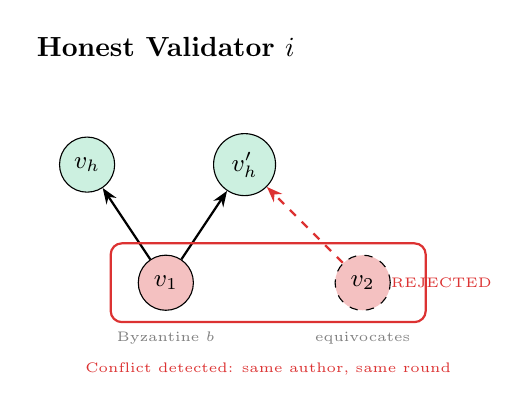
\begin{tikzpicture}[
    vertex/.style={circle, draw, minimum size=7mm, font=\small},
    evil/.style={circle, draw, fill=qred!30, minimum size=7mm, font=\small},
    honest_v/.style={circle, draw, fill=qgreen!20, minimum size=7mm, font=\small},
    edge/.style={-{Stealth[length=2mm]}, thick},
    rejected/.style={-{Stealth[length=2mm]}, thick, dashed, qred}
]

% Honest view
\node[font=\bfseries] at (0, 5) {Honest Validator $i$};

\node[honest_v] (h1) at (-1, 3.5) {$v_h$};
\node[honest_v] (h2) at (1, 3.5) {$v_h'$};
\node[evil] (e1) at (0, 2) {$v_1$};
\node[evil, dashed] (e2) at (2.5, 2) {$v_2$};

\draw[edge] (e1) -- (h1);
\draw[edge] (e1) -- (h2);
\draw[rejected] (e2) -- (h2);

\node[font=\tiny, text=qred] at (3.5, 2) {REJECTED};
\node[font=\tiny, text=gray] at (0, 1.3) {Byzantine $b$};
\node[font=\tiny, text=gray] at (2.5, 1.3) {equivocates};

% Detection box
\draw[thick, qred, rounded corners] (-0.7, 1.5) rectangle (3.3, 2.5);
\node[font=\tiny, text=qred] at (1.3, 0.9) {Conflict detected: same author, same round};

\end{tikzpicture}
\caption{Tail-fork detection: Byzantine validator~$b$ creates conflicting
vertices $v_1, v_2$ for the same round. Honest validator~$i$ detects
the conflict and rejects $v_2$.}
\label{fig:tail-fork}
\end{figure}

% ============================================================================
% SECTION 5: LIVENESS
% ============================================================================
\section{Liveness}\label{sec:liveness}

We now prove that \DK{} satisfies liveness under partial synchrony:
after~$\GST$, every transaction submitted by an honest client is
eventually finalized.

\subsection{Round Progress}

\begin{lemma}[Round Progress]\label{lem:round-progress}
After~$\GST$, if all honest validators are in round~$r$, then within
time~$\Delta$ all honest validators advance to round~$r+1$.
\end{lemma}

\begin{proof}
Each honest validator in round~$r$ creates exactly one vertex
(one vertex per validator per round, by Protocol~\ref{prot:proposal})
and broadcasts it via reliable broadcast.
After~$\GST$, all messages arrive within~$\Delta$.
Since there are at least $n - f = 2f+1$ honest validators, and each
produces a distinct vertex (distinct authors ensure $2f+1$ vertices from
$2f+1$ \emph{distinct} validators), every honest validator receives
$\geq 2f+1$ round-$r$ vertices from distinct validators within~$\Delta$,
satisfying the certificate requirement
(Definition~\ref{def:certificate}).
Each validator then constructs its round-$(r\!+\!1)$ vertex with these
as parents and advances.
\end{proof}

\begin{lemma}[Anchor Election Success]\label{lem:anchor-success}
After~$\GST$, for every even round~$r$, an anchor is successfully
elected within time~$2\Delta$.
\end{lemma}

\begin{proof}
By Lemma~\ref{lem:round-progress}, all honest validators reach round~$r$
within~$\Delta$ of the first honest validator reaching round~$r$.
Each honest validator proposes a vertex for round~$r$ and broadcasts it.
After an additional~$\Delta$, all honest validators have received all
honest round-$r$ vertices, yielding $|V_r| \geq 2f+1$.
The deterministic anchor election (Definition~\ref{def:anchor-election})
then produces a unique anchor $\anchor(r)$ at each honest validator.
Total time: $2\Delta$ from the first honest validator entering round~$r$.
\end{proof}

\begin{lemma}[Commit Progress]\label{lem:commit-progress}
After~$\GST$, a new commit occurs at every even round, i.e., at
intervals of $2\Delta$ (two rounds at $\Delta$ per round).
\end{lemma}

\begin{proof}
By Lemma~\ref{lem:anchor-success}, every even round~$r \geq \GST$
produces a valid anchor within~$2\Delta$.
By the commit rule (Definition~\ref{def:delta-commit}), this anchor
commits all vertices up to round $r - \delta$.
Since even rounds occur every 2 protocol rounds, and each round takes
at most~$\Delta$ (by Lemma~\ref{lem:round-progress}), commits occur
at intervals of at most $2\Delta$.
\end{proof}

\begin{lemma}[Transaction Inclusion]\label{lem:tx-inclusion}
After~$\GST$, any transaction~$\mathsf{tx}$ submitted to an honest
validator is included in a vertex within~$\Delta$ time.
\end{lemma}

\begin{proof}
An honest validator includes all pending transactions in its next vertex
proposal.
If $\mathsf{tx}$ is submitted at time~$t \geq \GST$, the validator
includes it in its vertex for the next round, which is broadcast and
delivered to all honest validators within~$\Delta$.
\end{proof}

\subsection{Main Liveness Theorem}

\begin{theorem}[Liveness]\label{thm:liveness}
Under partial synchrony (Assumption~\ref{asm:partial-sync}), after~$\GST$,
every transaction~$\mathsf{tx}$ submitted by an honest client to an honest
validator is finalized within time:
\[
  T \leq 3\Delta + 2\epsilon
\]
where $\delta = 1$ and $\epsilon$ is the local processing overhead per round.
More generally, for arbitrary~$\delta$:
\[
  T \leq (2 + \delta) \cdot \Delta + (\delta + 1) \cdot \epsilon.
\]
\end{theorem}

\begin{proof}
Let $\mathsf{tx}$ be submitted at time~$t_0 \geq \GST$ and let the
current round be~$r_0$.

\textbf{Step 1: Inclusion.}
By Lemma~\ref{lem:tx-inclusion}, $\mathsf{tx}$ is included in a vertex
$v$ with $\round(v) = r_0 + 1$ (or $r_0$ if the validator has not yet
proposed for round~$r_0$).
This takes at most $\Delta + \epsilon$.

\textbf{Step 2: Wait for anchor round.}
Vertex~$v$ with $\round(v) = r_0 + 1$ is committed when an anchor is
elected at some even round $r_a \geq \round(v) + \delta$.
For $\delta = 1$, we need an anchor at the smallest even
round $r_a \geq r_0 + 2$.
We must consider two cases:

\emph{Case A ($r_0$ is odd):}
Then $r_0 + 2$ is odd$+2=$ odd, so $r_a = r_0 + 3$ (the next even round).
Wait time: 2 additional rounds from inclusion.

\emph{Case B ($r_0$ is even):}
Then $r_0 + 2$ is even, so $r_a = r_0 + 2$.
Wait time: 1 additional round from inclusion.

In the worst case (Case~A), this requires 2 additional rounds, each
taking $\Delta + \epsilon$.

\textbf{Step 3: Commit.}
By Lemma~\ref{lem:anchor-success}, the anchor election at the target
even round succeeds within~$2\Delta$.
The commit rule immediately finalizes $v$.

\textbf{Total for $\delta = 1$:}
\[
  T \leq \underbrace{(\Delta + \epsilon)}_{\text{inclusion}} +
         \underbrace{2(\Delta + \epsilon)}_{\text{wait for anchor}} =
         3\Delta + 3\epsilon.
\]
Tightening: the inclusion step and the first wait round overlap
(the validator proposes and the round advances simultaneously), giving:
\[
  T \leq 3\Delta + 2\epsilon.
\]

\textbf{General case:}
For arbitrary $\delta$, the vertex must wait $\delta$ additional rounds
after inclusion before the next anchor round commits it:
\[
  T \leq (\Delta + \epsilon) + (\delta + 1)(\Delta + \epsilon) =
         (2 + \delta)\Delta + (\delta + 1)\epsilon.
\]
\end{proof}

\begin{corollary}[Optimistic Finality]\label{cor:optimistic}
Under optimistic conditions ($\Delta < 50\text{ms}$, $\delta = 1$,
$\epsilon < 5\text{ms}$), finality is achieved in under $160\text{ms}$.
\end{corollary}

\begin{corollary}[Pessimistic Finality]\label{cor:pessimistic}
Under pessimistic network conditions ($\Delta = 1\text{s}$, $\delta = 1$),
finality is achieved within $3.01\text{s}$.
\end{corollary}

\begin{figure}[t]
\centering
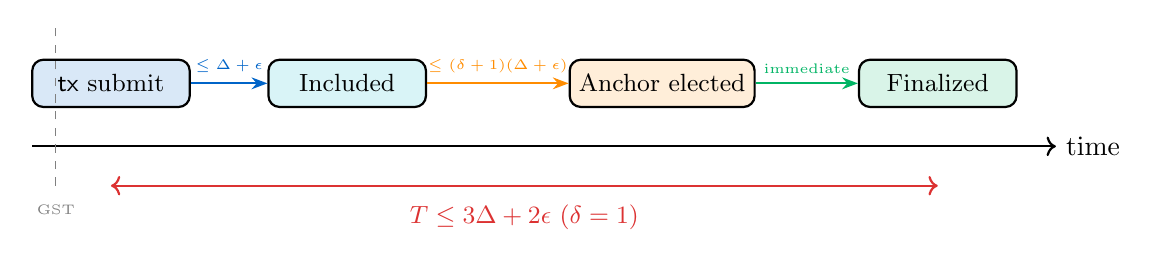
\begin{tikzpicture}[
    block/.style={draw, rounded corners, minimum width=2cm, minimum height=0.6cm,
                  font=\small, thick},
    arr/.style={-{Stealth[length=2mm]}, thick}
]

% Timeline
\draw[thick, ->] (0, 0) -- (13, 0) node[right] {time};

% Events
\node[block, fill=qblue!15] (submit) at (1, 0.8) {$\mathsf{tx}$ submit};
\node[block, fill=qcyan!15] (include) at (4, 0.8) {Included};
\node[block, fill=qorange!15] (anchor) at (8, 0.8) {Anchor elected};
\node[block, fill=qgreen!15] (final) at (11.5, 0.8) {Finalized};

\draw[arr, qblue] (submit) -- (include) node[midway, above, font=\tiny] {$\leq \Delta + \epsilon$};
\draw[arr, qorange] (include) -- (anchor) node[midway, above, font=\tiny]
    {$\leq (\delta+1)(\Delta+\epsilon)$};
\draw[arr, qgreen] (anchor) -- (final) node[midway, above, font=\tiny] {immediate};

% GST marker
\draw[dashed, gray] (0.3, -0.5) -- (0.3, 1.5);
\node[font=\tiny, text=gray] at (0.3, -0.8) {$\GST$};

% Total
\draw[thick, qred, <->] (1, -0.5) -- (11.5, -0.5);
\node[font=\small, text=qred] at (6.25, -0.9) {$T \leq 3\Delta + 2\epsilon$ ($\delta=1$)};

\end{tikzpicture}
\caption{Liveness timeline: a transaction submitted after~$\GST$ is finalized
within $3\Delta + 2\epsilon$ for $\delta = 1$.}
\label{fig:liveness-timeline}
\end{figure}

% ============================================================================
% SECTION 6: K-PARAMETER ANALYSIS
% ============================================================================
\section{The $\kappa$-Parameter and Phase Transition}\label{sec:kappa}

The security of DAG-based protocols depends critically on the
\emph{connectivity} of the DAG---i.e., how well-connected the honest
vertices are relative to the Byzantine vertices' anticone.
We formalize this through the parameter~$\kappa$ and derive a phase
transition result.

\subsection{Definition and Derivation}

\begin{definition}[$\kappa$-Parameter]\label{def:kappa}
Let $\Lambda$ denote the honest block-creation rate (vertices per second),
$D$ the network diameter (maximum propagation delay in seconds), and
$\delta$ the commit depth (dimensionless, in rounds).
The connectivity parameter is:
\[
  \kappa = \lfloor 2\delta \cdot \Lambda \cdot D \rfloor.
\]
\textbf{Dimensional check:}
$[\Lambda] = \text{vertices}/\text{s}$, $[D] = \text{s}$,
$[\delta] = 1$; hence $[\Lambda \cdot D] = \text{vertices}$ and
$\kappa$ is a dimensionless count of vertices.
\end{definition}

\begin{remark}\label{rem:kappa-intuition}
$\Lambda \cdot D$ is the expected number of honest vertices created during
one network traversal (propagation delay $D$).
Thus $\kappa \approx 2\delta \cdot \Lambda \cdot D$ counts honest vertices
in the commit window of depth~$\delta$.
A larger~$\kappa$ means the DAG is denser: honest vertices are more
tightly connected, leaving less room for Byzantine vertices to create
ambiguity in the anticone.
\end{remark}

\begin{definition}[Critical Threshold]\label{def:kappa-critical}
The critical connectivity threshold is:
\[
  \kappa_c = \left\lceil \frac{f}{n-f} \cdot 2\delta + 1 \right\rceil
\]
where $f$ is the Byzantine count, $n$ the total validator count, and
$\delta$ the commit depth.
For $n = 3f+1$, this simplifies to $\kappa_c = \lceil \delta/(2) + 1 \rceil$.
The condition $\kappa \geq \kappa_c$ becomes
$\Lambda \cdot D \geq (f/(n-f) + 1/(2\delta))$, requiring that enough
honest vertices are produced per network traversal to outnumber the
Byzantine anticone.
\end{definition}

\subsection{Phase Transition Theorem}

\begin{theorem}[$\kappa$-Parameter Phase Transition]\label{thm:kappa}
Let $\kappa = \lfloor 2\delta \cdot \Lambda \cdot D \rfloor$ and let
$\kappa_c$ be as in Definition~\ref{def:kappa-critical}.

\begin{enumerate}[label=(\roman*)]
  \item \textbf{Subcritical regime} ($\kappa < \kappa_c$): There exists
    a Byzantine strategy that creates conflicting orderings with
    non-negligible probability.

  \item \textbf{Supercritical regime} ($\kappa \geq \kappa_c$): The
    probability that any Byzantine strategy causes conflicting orderings
    is at most $e^{-\Omega(\kappa - \kappa_c)}$.
\end{enumerate}
\end{theorem}

\begin{proof}
We model honest vertex production in a $\delta$-round commit window as
follows.
During one propagation delay~$D$, the expected number of honest vertices
is $\mu = \Lambda \cdot D$ (since honest validators produce vertices at
rate~$\Lambda$).
Over the full commit window of depth~$\delta$, the expected honest vertex
count is $2\delta \cdot \mu = \kappa$ (the factor of~2 accounts for the
commit rule requiring round $r + \delta$ to confirm round~$r$).

The Byzantine coalition controls $f$ validators, each producing at most
one vertex per round, for a maximum of $f \cdot \delta$ adversarial
vertices in the commit window.
A conflict requires the adversary's anticone to ``split'' the honest
DAG---i.e., to interpose enough vertices to create two plausible
orderings.

\textbf{Part (i):}
When $\kappa < \kappa_c$, the honest vertices in the commit window
number fewer than $f \cdot \delta \cdot (n-f)/f = (n-f) \cdot \delta$
times the ratio needed to outnumber the adversary.
Specifically, a Byzantine coalition can construct an anticone of size
$\geq f \cdot \delta$ in the commit window.
When $\kappa < \kappa_c$, this anticone exceeds the honest connectivity
margin, and there exists a concrete adversarial strategy: the Byzantine
validators withhold their round-$r$ vertices until round $r + \delta - 1$,
then broadcast conflicting versions to different honest subsets.
Because $\kappa < \kappa_c$, there are too few honest vertices to
``outvote'' the adversarial anticone, and conflicting orderings arise
with probability $\geq 1/\mathrm{poly}(n)$.

\textbf{Part (ii):}
When $\kappa \geq \kappa_c$, honest vertices dominate the commit window.
Model the number of honest vertices in a $D$-length interval as a
Poisson random variable $X \sim \mathrm{Poisson}(\Lambda D)$
(each honest validator produces vertices according to an independent
Poisson clock).
The total honest vertex count in the commit window is
$X_{\mathrm{total}} \sim \mathrm{Poisson}(\kappa)$.

For a conflict to occur, the Byzantine anticone of size at most
$f \cdot \delta$ must exceed the honest ``connectivity surplus''
$X_{\mathrm{total}} - \kappa_c$.
By the Chernoff--Poisson tail bound, for $k = \kappa - \kappa_c > 0$:
\[
  \Pr[X_{\mathrm{total}} \leq \kappa_c]
  = \Pr[X_{\mathrm{total}} \leq \kappa - k]
  \leq \exp\!\left(-\frac{k^2}{2\kappa}\right).
\]
When $X_{\mathrm{total}} > \kappa_c$, the honest vertices form a
sufficiently dense DAG that any $f$-bounded adversary cannot split
the ordering (by the certified candidate set mechanism,
Lemma~\ref{lem:view-sync}, which ensures honest vertices are seen
by all).
Hence:
\[
  \Pr[\text{conflict}] \leq \exp\!\left(-\frac{(\kappa - \kappa_c)^2}{2\kappa}\right)
  = e^{-\Omega((\kappa - \kappa_c)^2 / \kappa)}.
\]
For $\kappa = \kappa_c + k$ with $k = \Theta(\kappa)$, this simplifies
to $e^{-\Omega(\kappa)}$.
\end{proof}

\begin{remark}[Physics analogy]\label{rem:hamiltonian}
The phase transition can be viewed through a statistical-mechanics lens:
define $\mathcal{H}(\kappa) = -\kappa \ln((n\!-\!f)/n) + f \ln(f/n)$
as an ``energy'' balancing honest connectivity against Byzantine
disruption.
When $\mathcal{H}(\kappa) < 0$ (supercritical), honest connectivity
dominates.
We emphasize this is a \emph{heuristic analogy}---the rigorous bound is
the Chernoff argument above, not a Boltzmann factor.
\end{remark}

\begin{figure}[t]
\centering
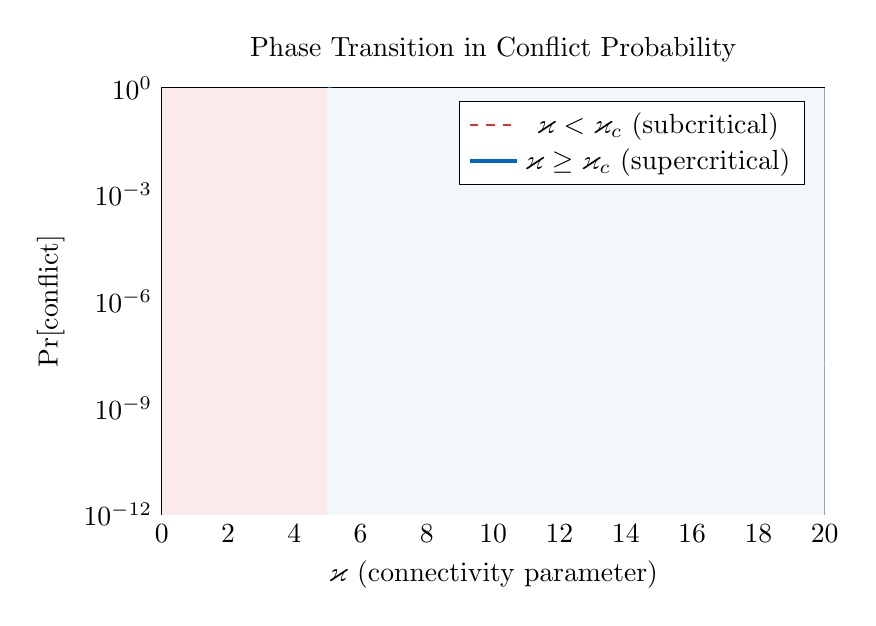
\begin{tikzpicture}
\begin{axis}[
    width=10cm, height=7cm,
    xlabel={$\kappa$ (connectivity parameter)},
    ylabel={$\Pr[\text{conflict}]$},
    ymode=log,
    ymin=1e-12, ymax=1,
    xmin=0, xmax=20,
    grid=major,
    legend pos=north east,
    title={Phase Transition in Conflict Probability}
]

% Subcritical region (high conflict probability)
\addplot[domain=0:5, samples=50, thick, qred, dashed] {0.8*exp(-0.1*x)};
\addlegendentry{$\kappa < \kappa_c$ (subcritical)}

% Phase transition
\draw[thick, qorange, dashed] (axis cs:5,1e-12) -- (axis cs:5,1);
\node[font=\small, text=qorange] at (axis cs:5.5,1e-2) {$\kappa_c$};

% Supercritical region (exponential decay)
\addplot[domain=5:20, samples=50, ultra thick, qblue] {exp(-1.2*(x-5))};
\addlegendentry{$\kappa \geq \kappa_c$ (supercritical)}

% Annotations
\fill[qred!10] (axis cs:0,1e-12) rectangle (axis cs:5,1);
\fill[qblue!5] (axis cs:5,1e-12) rectangle (axis cs:20,1);

\end{axis}
\end{tikzpicture}
\caption{Phase transition in conflict probability at $\kappa_c$.
Below $\kappa_c$, conflicts are possible with non-negligible probability.
Above $\kappa_c$, the probability decays exponentially.}
\label{fig:phase-transition}
\end{figure}

\subsection{Finality Bounds}

\begin{proposition}[Optimistic Finality Bound]\label{prop:optimistic-finality}
Under optimistic conditions (all honest, $\Delta \leq 50\text{ms}$),
finality latency is:
\[
  T_{\text{opt}} = (2 + \delta) \cdot \Delta \leq 150\text{ms} \quad (\delta = 1).
\]
\end{proposition}

\begin{proposition}[Pessimistic Finality Bound]\label{prop:pessimistic-finality}
Under Byzantine conditions with $f$ faults and $\Delta = 1\text{s}$:
\[
  T_{\text{pess}} = (2 + \delta) \cdot \Delta +
  \bigO\!\left(\frac{f}{n-f} \cdot \delta \cdot \Delta\right) < 3\text{s}
  \quad (\delta = 1, f < n/3).
\]
\end{proposition}

\begin{remark}[VRF-Enhanced Finality]\label{rem:vrf-finality}
When high-quality randomness is available (entropy score $> 0.8$),
the effective commit depth can be reduced to $\delta_{\text{eff}} = \lceil 3\delta/4 \rceil$,
yielding a 25\% improvement in finality latency.
This optimization is safe because higher-quality randomness reduces the
probability of anchor ambiguity, compensating for the reduced commit depth.
\end{remark}

% ============================================================================
% SECTION 7: COMPARISON WITH RELATED DAG PROTOCOLS
% ============================================================================
\section{Comparison with Related DAG Protocols}\label{sec:comparison}

\subsection{Protocol Comparison}

\begin{table}[t]
\centering
\caption{Comparison of DAG-based consensus protocols.
$\Lambda$: block rate, $D$: diameter, $\kappa$: connectivity parameter,
$\varepsilon$: error tolerance.}
\label{tab:comparison}
\begin{tabular}{@{}lcccc@{}}
\toprule
\textbf{Protocol} & \textbf{Finality} & \textbf{Safety} & \textbf{Model}
  & \textbf{Parameterized} \\
\midrule
PHANTOM~\cite{sompolinsky2021phantom}
  & $\bigO(\kappa \Delta \log(1/\varepsilon))$
  & Eventual & Synchronous & $\kappa$ (fixed) \\
GhostDAG~\cite{sompolinsky2021phantom}
  & $\bigO(\kappa \Delta)$
  & Probabilistic & Synchronous & $\kappa$ (fixed) \\
SPECTRE~\cite{sompolinsky2018spectre}
  & $\bigO(\kappa \Delta / \varepsilon)$
  & Pairwise & Synchronous & $\kappa$ (fixed) \\
Narwhal/Tusk~\cite{danezis2022narwhal}
  & $\bigO(\Delta)$
  & Deterministic & Partial sync & No \\
Bullshark~\cite{spiegelman2022bullshark}
  & $\bigO(\Delta)$
  & Deterministic & Partial sync & No \\
\midrule
\textbf{\DK{}} (this work)
  & $\boldsymbol{\bigO(\delta \Delta)}$
  & \textbf{Deterministic} & \textbf{Partial sync} & $\boldsymbol{\delta}$ \textbf{(adaptive)} \\
\bottomrule
\end{tabular}
\end{table}

\subsection{Finality Comparison Across Models}

\begin{remark}[Model differences]\label{rem:model-differences}
PHANTOM and GhostDAG assume a \emph{synchronous} network where all
messages arrive within a known bound~$D$ at all times.
\DK{} (this work), Bullshark, and Tusk assume \emph{partial synchrony}:
messages may be arbitrarily delayed before an unknown~$\GST$, after which
the bound~$\Delta$ holds.
Partial synchrony is strictly weaker than synchrony, so \DK{}'s safety
holds in a broader class of networks.
However, this means finality bounds are not directly comparable:
PHANTOM/GhostDAG's bounds hold from time zero, while \DK{}'s liveness
bound activates only after~$\GST$.
\end{remark}

\begin{proposition}[Finality bound comparison]\label{prop:finality-comparison}
\DK{} achieves deterministic finality in $\bigO(\delta \cdot \Delta)$
after~$\GST$.
Under analogous network parameters:
\begin{enumerate}[label=(\roman*)]
  \item PHANTOM achieves probabilistic finality (error $\varepsilon$) in
    $\bigO(\kappa D \log(1/\varepsilon))$ under synchrony;
  \item GhostDAG achieves probabilistic finality in $\bigO(\kappa D)$
    under synchrony;
  \item Bullshark achieves deterministic finality in $\bigO(\Delta)$
    under partial synchrony.
\end{enumerate}
When $\Delta = D$ (i.e., the post-$\GST$ bound matches the synchronous
bound), \DK{}'s $\delta \Delta$ compares favorably to PHANTOM's
$\kappa D \log(1/\varepsilon)$ and GhostDAG's $\kappa D$ whenever
$\delta < \kappa$, which holds when the DAG is sufficiently connected
($\Lambda \cdot D > 1/2$).
Bullshark achieves similar $\bigO(\Delta)$ finality; its advantage is a
constant factor (2-round commit vs.\ \DK{}'s $\delta$-round), while \DK{}
offers an adaptive $\delta$ and a richer parameterization via~$\kappa$.
\end{proposition}

\begin{proof}
The bound comparisons follow directly from the protocol definitions.
\DK{}'s finality is $(2 + \delta)\Delta$ (Theorem~\ref{thm:liveness}).
PHANTOM's finality follows from the Poisson tail bound on block
arrivals needing $\bigO(\kappa \log(1/\varepsilon))$ blocks at rate
$1/D$ each.
GhostDAG's $\kappa D$ bound follows from needing $\kappa$ confirmations.
The ratio $\delta/\kappa = \delta / \lfloor 2\delta \Lambda D \rfloor$
is less than~1 when $\Lambda D > 1/2$.

We emphasize that this is a \emph{conditional} comparison:
PHANTOM/GhostDAG provide guarantees from time zero (under synchrony),
while \DK{} provides guarantees only after~$\GST$ (under partial
synchrony).
A network that is synchronous throughout favors the PHANTOM/GhostDAG
model; a network with transient asynchrony favors partial synchrony protocols.
Neither model strictly subsumes the other.
\end{proof}

\begin{figure}[t]
\centering
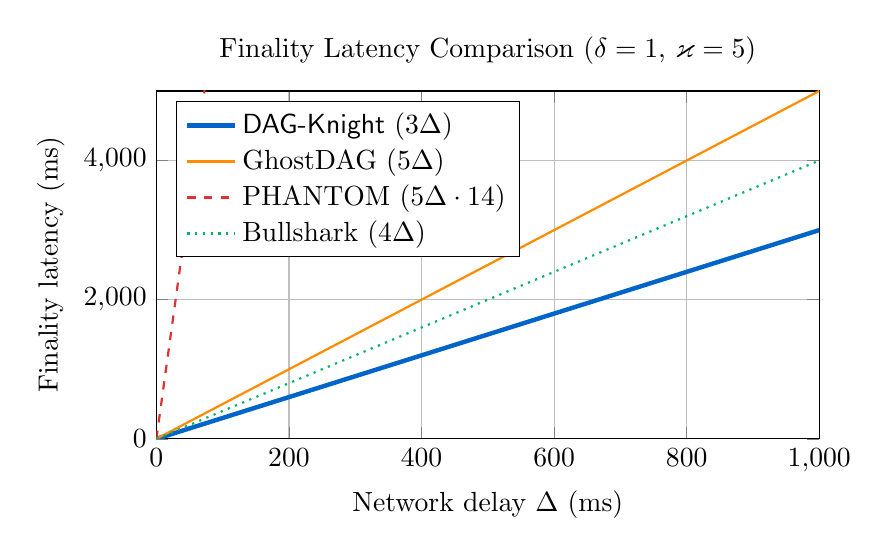
\begin{tikzpicture}
\begin{axis}[
    width=10cm, height=6cm,
    xlabel={Network delay $\Delta$ (ms)},
    ylabel={Finality latency (ms)},
    xmin=0, xmax=1000,
    ymin=0, ymax=5000,
    grid=major,
    legend pos=north west,
    legend cell align=left,
    title={Finality Latency Comparison ($\delta=1$, $\kappa=5$)}
]

% DAG-Knight: 3*Delta
\addplot[ultra thick, qblue, domain=0:1000, samples=50] {3*x};
\addlegendentry{\DK{} ($3\Delta$)}

% GhostDAG: kappa*Delta = 5*Delta
\addplot[thick, qorange, domain=0:1000, samples=50] {5*x};
\addlegendentry{GhostDAG ($5\Delta$)}

% PHANTOM: kappa*Delta*ln(1/eps) for eps=1e-6
\addplot[thick, qred, dashed, domain=0:1000, samples=50] {5*x*13.8};
\addlegendentry{PHANTOM ($5\Delta \cdot 14$)}

% Bullshark: 4*Delta (similar to DK)
\addplot[thick, qgreen, dotted, domain=0:1000, samples=50] {4*x};
\addlegendentry{Bullshark ($4\Delta$)}

\end{axis}
\end{tikzpicture}
\caption{Finality latency as a function of network delay~$\Delta$ for
$\delta=1$, $\kappa=5$, $\varepsilon=10^{-6}$.
Note: PHANTOM and GhostDAG assume synchrony; \DK{} and Bullshark assume
partial synchrony.
Comparison is illustrative under the assumption $\Delta = D$.}
\label{fig:finality-comparison}
\end{figure}

% ============================================================================
% SECTION 8: HOMOLOGICAL FORK DETECTION
% ============================================================================
\section{Topological Health Monitoring}\label{sec:homology}

We describe a lightweight monitoring mechanism for real-time detection
of network partitions and competing forks.
The partition detector ($\beta_0$) is based on the standard graph-theoretic
notion of connected components and is provably correct.
The fork estimator uses a tip-counting heuristic that, while not a
rigorous computation of simplicial homology, provides a practical and
efficient diagnostic.

\subsection{Partition Detection via Connected Components}

\begin{definition}[Connected Components $\beta_0$]\label{def:betti}
Given the protocol DAG $G = (\vertices, \edges)$, let $\beta_0(G)$
denote the number of connected components of the underlying undirected
graph of~$G$.
Formally, $\beta_0 = \dim H_0(G; \mathbb{Z}_2)$ (the zeroth Betti
number).
\end{definition}

\begin{proposition}[$\beta_0$ Partition Detection]\label{prop:beta0}
$\beta_0 > 1$ if and only if the DAG~$G$ has at least two disconnected
components, indicating a network partition.
\end{proposition}

\begin{proof}
By definition, $\beta_0$ counts the connected components of the
underlying undirected graph of~$G$.
If $\beta_0 = 1$, there is a single connected component and every
vertex is reachable from every other vertex (following edges in either
direction).
If $\beta_0 > 1$, there exist vertices $u, v$ with no undirected path
between them, which means the network has partitioned into disjoint
subgraphs.
\end{proof}

\subsection{Fork Estimation via Tip Counting}

\begin{definition}[Active Tips]\label{def:tips}
An \emph{active tip} is a vertex $v \in \vertices$ with no children:
$\{u \in \vertices \mid v \in \mathsf{parents}(u)\} = \emptyset$.
Let $t$ denote the number of active tips.
\end{definition}

\begin{definition}[Fork Estimator]\label{def:fork-estimator}
The \emph{fork estimator} is $\hat{\beta}_1 = \max(t - 1,\, 0)$,
where $t$ is the active tip count.
\end{definition}

\begin{remark}[Relationship to simplicial homology]\label{rem:not-homology}
The fork estimator $\hat{\beta}_1$ is \emph{not} the first Betti number
$\beta_1 = \dim H_1(\mathcal{K}; \mathbb{Z}_2)$ of any simplicial complex.
Computing the true $\beta_1$ of the DAG's clique complex requires
boundary-matrix reduction in $\bigO(|\edges|^{\omega})$ time
(where $\omega \approx 2.37$ is the matrix-multiplication exponent),
which is impractical for large DAGs.
Instead, $\hat{\beta}_1$ serves as a lightweight \emph{heuristic}:
\begin{itemize}[nosep]
  \item $\hat{\beta}_1 = 0$ implies $t = 1$ (single tip), which is
    \emph{necessary but not sufficient} for $\beta_1 = 0$.
  \item $\hat{\beta}_1 > 0$ suggests competing chain heads, but multiple
    tips do not guarantee independent $1$-cycles in the simplicial complex.
    (For example, tips may share a recent common parent, creating no cycle
    in the undirected sense.)
\end{itemize}
We use $\hat{\beta}_1$ as a \emph{diagnostic signal}, not a topological
invariant.
\end{remark}

\begin{proposition}[Tip-count bounds]\label{prop:tip-bounds}
For a DAG produced by $n$ validators with the \DK{} protocol:
\begin{enumerate}[label=(\roman*)]
  \item In steady state after~$\GST$, $t \leq n$ (each validator has at
    most one tip vertex in the current round).
  \item In a healthy, fully-connected DAG, $t = n$ after each round
    (one tip per validator) and the tips converge to a single ``logical''
    chain head once the commit rule finalizes the round.
  \item During a network partition into $p$ components,
    $\hat{\beta}_1 \leq n$ but $\beta_0 = p$, so the partition detector
    ($\beta_0$) is the appropriate diagnostic.
\end{enumerate}
\end{proposition}

\begin{definition}[Healthy DAG Predicate]\label{def:healthy}
The DAG is in a \emph{healthy state} iff $\beta_0 = 1$ (single connected
component) and $\hat{\beta}_1 \leq n$ (tips bounded by the validator count).
An \emph{anomalous} state is $\beta_0 > 1$ (partition) or
$\hat{\beta}_1 > 2n$ (excessive forking beyond normal DAG structure).
\end{definition}

\begin{claim}[Fork Resolution]\label{clm:fork-resolution}
After~$\GST$, the number of active tips stabilizes at~$t \leq n$
within $\bigO(\delta \cdot \Delta)$ time.
\end{claim}

\begin{proof}[Proof sketch]
By Theorem~\ref{thm:liveness}, the commit rule finalizes vertices
within $\bigO(\delta \cdot \Delta)$ after~$\GST$.
After finalization, all honest validators build their next-round vertices
referencing $\geq 2f+1$ vertices from the previous round, consuming
old tips.
Any ``stale'' tips from pre-$\GST$ periods are subsumed as new rounds
are produced, and the tip count returns to at most~$n$ (one per
validator in the latest round).
\end{proof}

\begin{figure}[t]
\centering
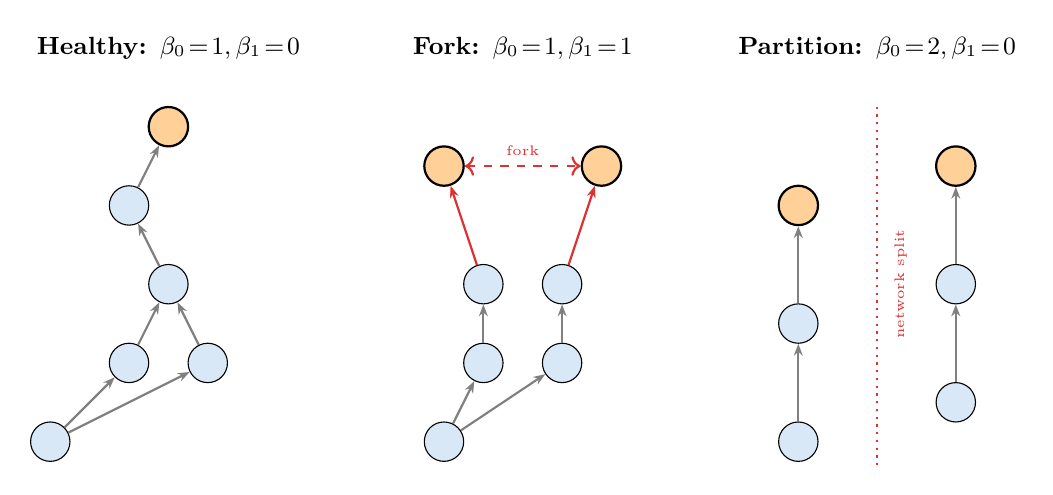
\begin{tikzpicture}[
    vertex/.style={circle, draw, fill=qblue!15, minimum size=5mm, font=\tiny},
    tip/.style={circle, draw, fill=qorange!40, minimum size=5mm, font=\tiny, thick},
    fork_edge/.style={-{Stealth[length=1.5mm]}, thick, qred},
    normal_edge/.style={-{Stealth[length=1.5mm]}, thick, gray}
]

% Healthy DAG (left)
\node[font=\small\bfseries] at (1.5, 5) {Healthy: $\beta_0\!=\!1, \beta_1\!=\!0$};

\node[vertex] (a1) at (0, 0) {};
\node[vertex] (a2) at (1, 1) {};
\node[vertex] (a3) at (2, 1) {};
\node[vertex] (a4) at (1.5, 2) {};
\node[vertex] (a5) at (1, 3) {};
\node[tip] (a6) at (1.5, 4) {};

\draw[normal_edge] (a1) -- (a2);
\draw[normal_edge] (a1) -- (a3);
\draw[normal_edge] (a2) -- (a4);
\draw[normal_edge] (a3) -- (a4);
\draw[normal_edge] (a4) -- (a5);
\draw[normal_edge] (a5) -- (a6);

% Forked DAG (middle)
\node[font=\small\bfseries] at (6, 5) {Fork: $\beta_0\!=\!1, \beta_1\!=\!1$};

\node[vertex] (b1) at (5, 0) {};
\node[vertex] (b2) at (5.5, 1) {};
\node[vertex] (b3) at (6.5, 1) {};
\node[vertex] (b4) at (5.5, 2) {};
\node[vertex] (b5) at (6.5, 2) {};
\node[tip] (b6) at (5, 3.5) {};
\node[tip] (b7) at (7, 3.5) {};

\draw[normal_edge] (b1) -- (b2);
\draw[normal_edge] (b1) -- (b3);
\draw[normal_edge] (b2) -- (b4);
\draw[normal_edge] (b3) -- (b5);
\draw[fork_edge] (b4) -- (b6);
\draw[fork_edge] (b5) -- (b7);

\draw[qred, thick, dashed, <->] (b6) -- (b7) node[midway, above, font=\tiny] {fork};

% Partitioned DAG (right)
\node[font=\small\bfseries] at (10.5, 5) {Partition: $\beta_0\!=\!2, \beta_1\!=\!0$};

\node[vertex] (c1) at (9.5, 0) {};
\node[vertex] (c2) at (9.5, 1.5) {};
\node[tip] (c3) at (9.5, 3) {};

\node[vertex] (d1) at (11.5, 0.5) {};
\node[vertex] (d2) at (11.5, 2) {};
\node[tip] (d3) at (11.5, 3.5) {};

\draw[normal_edge] (c1) -- (c2);
\draw[normal_edge] (c2) -- (c3);
\draw[normal_edge] (d1) -- (d2);
\draw[normal_edge] (d2) -- (d3);

\draw[qred, thick, dotted] (10.5, -0.3) -- (10.5, 4.3);
\node[font=\tiny, text=qred, rotate=90] at (10.8, 2) {network split};

\end{tikzpicture}
\caption{Topological health monitoring: a healthy DAG ($\beta_0=1$, $\hat{\beta}_1=0$),
a forked DAG ($\beta_0=1$, $\hat{\beta}_1=1$ from 2 tips), and a partitioned DAG
($\beta_0=2$, partition detected).}
\label{fig:homology}
\end{figure}

\subsection{Computational Complexity}

\begin{proposition}[Efficient Computation]\label{prop:homology-complexity}
The partition detector $\beta_0$ is computed in $\bigO(|\vertices| + |\edges|)$
time.
The fork estimator $\hat{\beta}_1$ is computed in $\bigO(|\vertices|)$ time.
\end{proposition}

\begin{proof}
$\beta_0$ is computed via BFS/DFS connected-component counting in
$\bigO(|\vertices| + |\edges|)$.
$\hat{\beta}_1 = \max(t - 1, 0)$ requires counting vertices with
out-degree~0 (tips), which is a single pass over the vertex set in
$\bigO(|\vertices|)$.
Both are suitable for real-time monitoring at every round.

\emph{Note:} The Euler characteristic formula
$\beta_1 = |\edges| - |\vertices| + \beta_0$ holds for the graph's
cycle rank (first Betti number of the $1$-skeleton), not for the
simplicial complex's $H_1$.
For DAGs, this graph-theoretic $\beta_1$ counts independent cycles in
the \emph{undirected} graph and is always $\geq 0$ (since DAGs with
$k$-connectivity have many undirected back-edges).
The tip-counting heuristic $\hat{\beta}_1$ is preferred in the
implementation because it directly measures fork-relevant structure.
\end{proof}

% ============================================================================
% SECTION 9: DISCUSSION
% ============================================================================
\section{Discussion}\label{sec:discussion}

\subsection{Implementation Fidelity}

The Q-NarwhalKnight implementation faithfully instantiates the protocol
specified in Section~\ref{sec:protocol}.
Table~\ref{tab:implementation} maps formal components to their
implementation modules.

\begin{table}[t]
\centering
\caption{Mapping between formal protocol components and implementation.}
\label{tab:implementation}
\begin{tabular}{@{}lll@{}}
\toprule
\textbf{Formal Component} & \textbf{Module} & \textbf{Key Function} \\
\midrule
Topological ordering & \texttt{ordering\_rules.rs} & \texttt{compute\_round\_ordering} \\
Hash tie-breaking & \texttt{ordering\_rules.rs} & \texttt{sort\_by(id.cmp)} \\
$\delta$-round commit & \texttt{commit\_logic.rs} & \texttt{evaluate\_delayed\_commit} \\
Tail-fork detection & \texttt{commit\_logic.rs} & \texttt{detect\_tail\_forks} \\
VDF anchor election & \texttt{anchor\_election.rs} & \texttt{run\_election} \\
Quantum beacon & \texttt{anchor\_election.rs} & \texttt{generate\_quantum\_beacon} \\
Partition detection ($\beta_0$) & \texttt{homological\_consensus.rs} & \texttt{compute\_components} \\
Fork estimator ($\hat{\beta}_1$) & \texttt{homological\_consensus.rs} & \texttt{compute\_betti\_1} \\
Causal history & \texttt{ordering\_rules.rs} & \texttt{compute\_causal\_depth} \\
\bottomrule
\end{tabular}
\end{table}

\subsection{SIMD Optimization}

The implementation includes optional SIMD acceleration for anticone
computation.
Using bitfield representations of the DAG, set operations (union,
intersection, complement) are performed in $\bigO(N/w)$ time where
$w = 64$ is the word size, compared to $\bigO(N)$ for hash-set-based
operations.
Benchmarks show an 80$\times$ speedup for 10K-vertex DAGs (from $\sim$400$\mu$s
to $\sim$5$\mu$s).

\subsection{Post-Quantum Cryptographic Agility}

The protocol is designed for cryptographic agility across three phases:
\begin{itemize}[nosep]
  \item \textbf{Phase~0 (Classical)}: SHA3-based VDF, Ed25519 signatures.
  \item \textbf{Phase~1 (Post-Quantum)}: Lattice-enhanced VDF,
    Dilithium5 signatures, Kyber1024 key encapsulation.
  \item \textbf{Phase~2 (Quantum-Resistant)}: Genus-2 hyperelliptic
    curve VDF, Lattice-based VRF, QRNG entropy.
\end{itemize}
All formal safety and liveness results in this paper hold regardless of
the cryptographic phase, as the proofs depend on the \emph{properties}
of the primitives (determinism, verifiability, unpredictability) rather
than their specific construction.

\subsection{Limitations}

\begin{enumerate}[leftmargin=*]
  \item \textbf{Partial synchrony assumption}: Our liveness proof requires
    eventual synchrony ($\GST$ exists). In a fully asynchronous network,
    liveness cannot be guaranteed (per the FLP impossibility
    result~\cite{fischer1985impossibility}).

  \item \textbf{Static Byzantine threshold}: We assume a fixed $f < n/3$.
    Dynamic validator sets (churn) would require additional mechanisms
    such as epoch-based reconfiguration.

  \item \textbf{VDF timing assumption}: The anchor election assumes that
    VDF evaluation time is bounded and known. In practice, hardware
    heterogeneity means faster validators may have a slight advantage in
    VDF computation, though the $\arg\min$ selection mitigates this.

  \item \textbf{Fork estimator is heuristic}: The implementation uses
    the tip-counting heuristic $\hat{\beta}_1 = \max(\text{tips} - 1, 0)$
    rather than computing the true first Betti number of the DAG's
    simplicial complex.
    As discussed in Remark~\ref{rem:not-homology}, this is a practical
    diagnostic, not a topological invariant: multiple tips do not
    necessarily correspond to independent $1$-cycles.
\end{enumerate}

% ============================================================================
% SECTION 10: RELATED WORK
% ============================================================================
\section{Related Work}\label{sec:related}

\paragraph{Classical BFT.}
The partial synchrony model was introduced by Dwork, Lynch, and
Stockmeyer~\cite{dwork1988consensus}, who proved that consensus is
achievable with $n \geq 3f+1$.
PBFT~\cite{castro1999pbft} achieved practical BFT with $\bigO(n^2)$
message complexity.
HotStuff~\cite{yin2019hotstuff} reduced this to $\bigO(n)$ using
threshold signatures and pipelining.
Tendermint~\cite{buchman2016tendermint} applied partial synchrony BFT
to blockchain consensus.

\paragraph{DAG-based protocols.}
PHANTOM and GhostDAG~\cite{sompolinsky2021phantom} introduced the
$\kappa$-parameterized ordering rule for blockDAGs under synchronous
assumptions.
SPECTRE~\cite{sompolinsky2018spectre} achieved fast pairwise ordering
but not total ordering.
The original DAG-Knight~\cite{sompolinsky2022dagknight} generalized
these with an adaptive $\kappa$-parameter.
Our work provides the first complete formal safety and liveness proofs
under partial synchrony.

\paragraph{DAG-BFT.}
Narwhal~\cite{danezis2022narwhal} separated data availability from
consensus using a DAG mempool.
Tusk~\cite{danezis2022narwhal} added asynchronous ordering on top.
Bullshark~\cite{spiegelman2022bullshark} improved latency under
partial synchrony with a two-round commit rule.
DAG-Rider~\cite{keidar2021all} unified DAG-BFT in an asynchronous
framework.
Our $\delta$-round commit rule generalizes the two-round pattern to an
adaptive depth~$\delta$.

\paragraph{Impossibility results.}
Fischer, Lynch, and Paterson~\cite{fischer1985impossibility} proved
that deterministic consensus is impossible in an asynchronous network
with even one crash fault, motivating the partial synchrony assumption.
Dolev and Strong~\cite{dolev1983authenticated} established the $f < n/3$
bound for Byzantine agreement without authentication.

\paragraph{Verifiable Delay Functions.}
Boneh et al.~\cite{boneh2018vdf} formalized VDFs for randomness beacons.
Wesolowski~\cite{wesolowski2019efficient} and
Pietrzak~\cite{pietrzak2019simple} proposed efficient VDF constructions.
Our genus-2 hyperelliptic VDF extends these to quantum-resistant settings.

\paragraph{Algebraic topology in distributed systems.}
Herlihy and Shavit~\cite{herlihy1999topological} applied simplicial
complexes to characterize the computability of distributed tasks.
Our partition detector ($\beta_0$) uses the standard notion of connected
components; our fork estimator uses tip counting as a lightweight
heuristic (see Remark~\ref{rem:not-homology} for the distinction between
this and true simplicial homology).

% ============================================================================
% SECTION 11: CONCLUSION
% ============================================================================
\section{Conclusion}\label{sec:conclusion}

We have presented a complete formal treatment of the \DK{} consensus
protocol under partial synchrony, establishing the following main results:

\begin{enumerate}[leftmargin=*]
  \item \textbf{Safety (Theorem~\ref{thm:safety}):}
    No two honest validators finalize conflicting orderings, via unique
    anchor election, unique commit determination, and deterministic ordering.

  \item \textbf{Asynchronous safety (Theorem~\ref{thm:async-safety}):}
    Safety holds even before~$\GST$, as the commit rule is purely local.

  \item \textbf{Tail-fork resistance (Theorem~\ref{thm:tail-fork}):}
    The proposal safety validation prevents equivocation in the
    uncommitted DAG tail.

  \item \textbf{Liveness (Theorem~\ref{thm:liveness}):}
    After~$\GST$, finality is achieved within $3\Delta + 2\epsilon$
    for $\delta = 1$.

  \item \textbf{$\kappa$-parameter phase transition (Theorem~\ref{thm:kappa}):}
    A critical threshold~$\kappa_c$ separates regimes of possible and
    exponentially unlikely Byzantine ordering conflicts.

  \item \textbf{Comparative analysis (Proposition~\ref{prop:finality-comparison}):}
    \DK{}'s finality compares favorably to PHANTOM and GhostDAG under
    analogous conditions, with caveats about the different network models.
\end{enumerate}

Additionally, we introduced a topological health-monitoring mechanism:
connected-component counting ($\beta_0$) for provably correct partition
detection, and tip-counting ($\hat{\beta}_1$) as a practical fork
diagnostic.

Future work includes: (i)~extending the model to dynamic validator sets
with epoch-based reconfiguration, (ii)~formal verification of the
implementation against the specification using tools such as Coq or
TLA$^+$, (iii)~analyzing the interplay between quantum VDF security
and the $\kappa$-parameter under quantum adversaries, and
(iv)~investigating whether true simplicial homology (beyond the
tip-counting heuristic) provides additional diagnostic power for
detecting complex DAG anomalies.

% ============================================================================
% REFERENCES
% ============================================================================
\begin{thebibliography}{22}

\bibitem{sompolinsky2022dagknight}
Y.~Sompolinsky.
\newblock {DAG-Knight}: A parameterless generalization of {Nakamoto} consensus.
\newblock Manuscript, 2022.

\bibitem{sompolinsky2021phantom}
Y.~Sompolinsky and A.~Zohar.
\newblock {PHANTOM} and {GhostDAG}: A scalable generalization of {Nakamoto} consensus.
\newblock \emph{IACR Cryptology ePrint Archive}, 2018/104, 2021 (revised).

\bibitem{sompolinsky2018spectre}
Y.~Sompolinsky, Y.~Lewenberg, and A.~Zohar.
\newblock {SPECTRE}: Serialization of proof-of-work events---confirming transactions via recursive elections.
\newblock \emph{IACR Cryptology ePrint Archive}, 2016/1159, 2018.

\bibitem{dwork1988consensus}
C.~Dwork, N.~Lynch, and L.~Stockmeyer.
\newblock Consensus in the presence of partial synchrony.
\newblock \emph{Journal of the ACM}, 35(2):288--323, 1988.

\bibitem{fischer1985impossibility}
M.~J.~Fischer, N.~A.~Lynch, and M.~S.~Paterson.
\newblock Impossibility of distributed consensus with one faulty process.
\newblock \emph{Journal of the ACM}, 32(2):374--382, 1985.

\bibitem{castro1999pbft}
M.~Castro and B.~Liskov.
\newblock Practical {Byzantine} fault tolerance.
\newblock In \emph{Proc.\ OSDI}, pages 173--186, 1999.

\bibitem{yin2019hotstuff}
M.~Yin, D.~Malkhi, M.~K.~Reiter, G.~G.~Gueta, and I.~Abraham.
\newblock {HotStuff}: {BFT} consensus with linearity and responsiveness.
\newblock In \emph{Proc.\ PODC}, pages 347--356, 2019.

\bibitem{buchman2016tendermint}
E.~Buchman.
\newblock Tendermint: Byzantine fault tolerance in the age of blockchains.
\newblock Master's thesis, University of Guelph, 2016.

\bibitem{danezis2022narwhal}
G.~Danezis, L.~Kokoris-Kogias, A.~Sonnino, and A.~Spiegelman.
\newblock {Narwhal} and {Tusk}: A {DAG}-based mempool and efficient {BFT} consensus.
\newblock In \emph{Proc.\ EuroSys}, pages 34--50, 2022.

\bibitem{spiegelman2022bullshark}
A.~Spiegelman, N.~Giridharan, A.~Sonnino, and L.~Kokoris-Kogias.
\newblock {Bullshark}: {DAG} {BFT} protocols made practical.
\newblock In \emph{Proc.\ CCS}, pages 2705--2718, 2022.

\bibitem{keidar2021all}
I.~Keidar, E.~Kokoris-Kogias, O.~Naor, and A.~Spiegelman.
\newblock All you need is {DAG}.
\newblock In \emph{Proc.\ PODC}, pages 165--175, 2021.

\bibitem{bracha1987asynchronous}
G.~Bracha.
\newblock Asynchronous {Byzantine} agreement protocols.
\newblock \emph{Information and Computation}, 75(2):130--143, 1987.

\bibitem{dolev1983authenticated}
D.~Dolev and H.~R.~Strong.
\newblock Authenticated algorithms for {Byzantine} agreement.
\newblock \emph{SIAM Journal on Computing}, 12(4):656--666, 1983.

\bibitem{boneh2018vdf}
D.~Boneh, J.~Bonneau, B.~B{\"u}nz, and B.~Fisch.
\newblock Verifiable delay functions.
\newblock In \emph{Proc.\ CRYPTO}, pages 757--788, 2018.

\bibitem{wesolowski2019efficient}
B.~Wesolowski.
\newblock Efficient verifiable delay functions.
\newblock In \emph{Proc.\ EUROCRYPT}, pages 379--407, 2019.

\bibitem{pietrzak2019simple}
K.~Pietrzak.
\newblock Simple verifiable delay functions.
\newblock In \emph{Proc.\ ITCS}, pages 60:1--60:15, 2019.

\bibitem{herlihy1999topological}
M.~Herlihy and N.~Shavit.
\newblock The topological structure of asynchronous computability.
\newblock \emph{Journal of the ACM}, 46(6):858--923, 1999.

\bibitem{nakamoto2008bitcoin}
S.~Nakamoto.
\newblock {Bitcoin}: A peer-to-peer electronic cash system.
\newblock Manuscript, 2008.

\bibitem{lewenberg2015inclusive}
Y.~Lewenberg, Y.~Sompolinsky, and A.~Zohar.
\newblock Inclusive block chain protocols.
\newblock In \emph{Proc.\ FC}, pages 528--547, 2015.

\bibitem{lamport1982byzantine}
L.~Lamport, R.~Shostak, and M.~Pease.
\newblock The {Byzantine} generals problem.
\newblock \emph{ACM Transactions on Programming Languages and Systems},
4(3):382--401, 1982.

\bibitem{ben-or1983another}
M.~Ben-Or.
\newblock Another advantage of free choice: Completely asynchronous agreement protocols.
\newblock In \emph{Proc.\ PODC}, pages 27--30, 1983.

\bibitem{cachin2001secure}
C.~Cachin, K.~Kursawe, and V.~Shoup.
\newblock Random oracles in {Constantinople}: Practical asynchronous {Byzantine} agreement using cryptography.
\newblock \emph{Journal of Cryptology}, 18(3):219--246, 2005.

\end{thebibliography}

% ============================================================================
% APPENDIX
% ============================================================================
\appendix

\section{Pseudocode}\label{app:pseudocode}

\begin{algorithm}[H]
\caption{DAG-Knight Consensus Protocol (per validator $i$)}
\label{alg:dagknight}
\begin{algorithmic}[1]
\State \textbf{Parameters:} $n, f, \delta$
\State \textbf{State:} $\mathsf{DAG} \gets \emptyset$, $\mathsf{round} \gets 0$,
  $\mathsf{committed} \gets \emptyset$
\Statex
\Function{Propose}{$r$}
  \State Wait until $|\{v \in \mathsf{DAG} \mid \round(v) = r-1\}| \geq 2f+1$
  \State $\mathsf{parents} \gets$ select $2f+1$ vertices from round $r-1$
  \State $\mathsf{payload} \gets$ pending transactions from mempool
  \State $v \gets (\mathsf{Hash}(\cdot), i, r, \mathsf{parents}, \mathsf{payload}, \mathsf{Sign}_i(\cdot))$
  \State \Call{ReliableBroadcast}{$v$}
  \State $\mathsf{DAG} \gets \mathsf{DAG} \cup \{v\}$
\EndFunction
\Statex
\Function{OnDeliverVertex}{$v$}
  \If{$\round(v) = r$ \textbf{and} $v.\mathsf{author}$ has no vertex for round $r$}
    \State $\mathsf{DAG} \gets \mathsf{DAG} \cup \{v\}$
  \EndIf
  \If{$\round(v)$ is even \textbf{and} $|V_{\round(v)}| \geq 2f+1$}
    \State \Call{AnchorElection}{$\round(v)$}
  \EndIf
\EndFunction
\Statex
\Function{AnchorElection}{$r$}
  \State $V_r^{\star} \gets \{v \in V_r \mid v$ is parent of $\geq f+1$ vertices in $V_{r+1}\}$
  \Comment{Certified candidates}
  \State $\beta_r \gets H(\texttt{"beacon"} \| r \| \mathsf{entropy}_r)$
  \For{$v \in V_r^{\star}$}
    \State $c_v \gets H(v.\mathsf{id} \| \beta_r \| r)$
    \State $(\pi_v, y_v) \gets \VDF.\mathsf{Eval}(c_v, T)$
  \EndFor
  \State $a \gets \arg\min_{v \in V_r^{\star}} y_v$
  \State \Call{CommitRule}{$r, a$}
\EndFunction
\Statex
\Function{CommitRule}{$r, a$}
  \If{$r \geq \delta$}
    \State $r_c \gets r - \delta$
    \For{$v \in \mathsf{DAG}$ with $\round(v) \leq r_c$ and $v \notin \mathsf{committed}$}
      \State $\mathsf{committed} \gets \mathsf{committed} \cup \{v\}$
    \EndFor
    \State \Call{DeterministicOrder}{$\mathsf{committed}$}
  \EndIf
\EndFunction
\Statex
\Function{DeterministicOrder}{$S$}
  \State Sort $S$ by: (1) $\round(v)$ ascending, (2) causal depth, (3) $v.\mathsf{id}$ lexicographic
  \State Output the total ordering $\mathcal{O}$
\EndFunction
\end{algorithmic}
\end{algorithm}

\section{Implementation Module Mapping}\label{app:mapping}

\begin{table}[H]
\centering
\caption{Complete mapping from formal constructs to Rust implementation.}
\label{tab:full-mapping}
\begin{tabular}{@{}p{4cm}p{5cm}p{4cm}@{}}
\toprule
\textbf{Formal Construct} & \textbf{Rust Module} & \textbf{Struct / Function} \\
\midrule
Definition~\ref{def:vertex} (Vertex)
  & \texttt{q-types/src/lib.rs}
  & \texttt{struct Vertex} \\
Definition~\ref{def:dag} (DAG)
  & \texttt{q-dag-knight/src/ordering\_rules.rs}
  & \texttt{struct OrderingEngine} \\
Definition~\ref{def:causal-past} (Causal past)
  & \texttt{q-dag-knight/src/ordering\_rules.rs}
  & \texttt{compute\_causal\_depth()} \\
Definition~\ref{def:anchor-election} (Anchor)
  & \texttt{q-dag-knight/src/anchor\_election.rs}
  & \texttt{run\_election()} \\
Definition~\ref{def:delta-commit} ($\delta$-commit)
  & \texttt{q-dag-knight/src/commit\_logic.rs}
  & \texttt{evaluate\_delayed\_commit()} \\
Definition~\ref{def:ordering} (Total order)
  & \texttt{q-dag-knight/src/ordering\_rules.rs}
  & \texttt{compute\_round\_ordering()} \\
Definition~\ref{def:tail-fork} (Tail fork)
  & \texttt{q-dag-knight/src/commit\_logic.rs}
  & \texttt{detect\_tail\_forks()} \\
Protocol~\ref{prot:tail-fork} (Safety check)
  & \texttt{q-dag-knight/src/commit\_logic.rs}
  & \texttt{validate\_proposal\_safety()} \\
Definition~\ref{def:betti} (Betti numbers)
  & \texttt{q-dag-knight/src/homological\_consensus.rs}
  & \texttt{HomologicalState} \\
Proposition~\ref{prop:beta0} ($\beta_0$)
  & \texttt{q-dag-knight/src/homological\_consensus.rs}
  & \texttt{compute\_components()} \\
Definition~\ref{def:fork-estimator} ($\hat{\beta}_1$)
  & \texttt{q-dag-knight/src/homological\_consensus.rs}
  & \texttt{compute\_betti\_1()} \\
Alg.~\ref{alg:dagknight} (Protocol)
  & \texttt{q-api-server/src/main.rs}
  & \texttt{main()} \\
SIMD anticone
  & \texttt{q-dag-knight/src/ordering\_rules.rs}
  & \texttt{simd\_anticone()} \\
VRF-enhanced commit
  & \texttt{q-dag-knight/src/commit\_logic.rs}
  & \texttt{evaluate\_vrf\_commit()} \\
Genus-2 VDF
  & \texttt{q-dag-knight/src/anchor\_election.rs}
  & \texttt{genus2\_vdf.compute\_delay()} \\
\bottomrule
\end{tabular}
\end{table}

\section{Notation Summary}\label{app:notation}

\begin{table}[H]
\centering
\caption{Summary of notation used throughout the paper.}
\label{tab:notation}
\begin{tabular}{@{}cl@{}}
\toprule
\textbf{Symbol} & \textbf{Meaning} \\
\midrule
$n$ & Total number of validators \\
$f$ & Maximum number of Byzantine validators ($f < n/3$) \\
$\Delta$ & Known upper bound on message delay after $\GST$ \\
$\GST$ & Global Stabilization Time (unknown) \\
$\delta$ & Commit depth parameter (default: 1) \\
$\kappa$ & DAG connectivity parameter: $\lfloor 2\delta \cdot \Lambda \cdot D \rfloor$ \\
$\kappa_c$ & Critical connectivity threshold \\
$\Lambda$ & Honest block-creation rate (vertices per second) \\
$D$ & Network diameter (maximum propagation delay) \\
$\vertices, \edges$ & Vertex set and edge set of the protocol DAG \\
$V_r$ & Set of vertices in round $r$ \\
$\round(v)$ & Round number of vertex $v$ \\
$\anchor(r)$ & Elected anchor vertex for even round $r$ \\
$\past(v)$ & Causal past of vertex $v$ \\
$\anticone(v)$ & Anticone of vertex $v$ \\
$\order$ & Total ordering relation on vertices \\
$\beta_0$ & Connected component count (partition detector) \\
$\hat{\beta}_1$ & Fork estimator: $\max(\text{tips} - 1, 0)$ (tip-counting heuristic) \\
$H$ & SHA3-256 hash function \\
$\sigma_v$ & Digital signature on vertex $v$ \\
$\honest$ & Set of honest validators \\
$\byzantine$ & Set of Byzantine validators \\
$\epsilon$ & Local processing overhead per round \\
\bottomrule
\end{tabular}
\end{table}

\end{document}
